\documentclass[
    headings=optiontohead,              % allows double headers
    12pt,                               % fontsize 
    DIV=13,                             % koma script diveider amount. tells koma how much of the site can be written to
    twoside=false,                      % if set to true, automatically formats as book style with different left and right pages
    open=right,                         % starting page on twosided texts 
    BCOR=00mm,                          % correction that accounts for the center of the pages being glued in
    toc=bibliographynumbered            % bibliography gets a number and is listed in the table of contents
]{scrreport}

\usepackage[english]{babel}                     % font that supports English
\usepackage{upgreek}                            % non-cursive Greek letters
\usepackage[stretch=10,shrink=10,protrusion=true,expansion=true,final]{microtype} % prettier block format
\usepackage{hyperref}                           % links for everything
\usepackage{color}                              % allows for setting in different colors
\usepackage[autooneside=false,automark]{scrlayer-scrpage} % page-style with "Kolumnentitel" (title of current chapter is displayed at the top)
\usepackage{amsfonts,amstext,amsmath,amsthm, amssymb} % better math mode (\mathrm and \text) and symbols
\usepackage[sb]{libertinus}                     % use the font libertinus (needs to be installed from the web)
%\usepackage[slantedGreek]{libertinust1math}     % math mode improvement for libertinus
\usepackage{siunitx}                            % physical units setting
\usepackage{icomma}                             % commas in lists get extra space if needed                        
\usepackage{xspace}                             % works to improve own commands and provides "\xspace"-command, that puts a space if needed
\usepackage{ifthen}                             % more control over non-obligatory parameters
\usepackage{titling}                            % get title values as macros
\usepackage[onehalfspacing]{setspace}           % control the spacing between lines and in enumeration lists
\usepackage[backend=biber, style=phys, biblabel=brackets, url=true]{biblatex} % citations with "modern" backend and an physics-accepted citation style
\usepackage{graphicx}                           % work with graphics 
\usepackage{ragged2e}                           % ragged-commands (when no block format is wanted)
\usepackage{pdfpages}                           % allows including of pdfs into this pdf
\usepackage{booktabs}                           % better table formatting
\usepackage{multicol}                           % allows for the definition of multi-columns in tables
\usepackage{multirow}                           % allows for the definition of multirow-tables instead of just multicolumn
\usepackage[section]{placeins}                  % provides the command "\FloatBarrier" to control the end of floatable regions for figures/tables
\usepackage{float}                              % provides the "H" option for forcing placement of a figure
\usepackage{floatpag}                           % make it possible for float-pages to not have a page number
\usepackage{url}                                % sometimes needed by biblatex, technically no longer needed
\usepackage{minted}                             % nice code highlighting (needs Python Package to compile!!)
\usepackage{mathtools}                          % more math control possibilities
\usepackage{eucal}                              % Different mathcal alphabet
\usepackage[autostyle=true]{csquotes}           % context-sensitive-quotes -> quotation marks that are set correctly for the context
\usepackage{physics}                            % bra-ket and more
\usepackage{nicematrix}                         % label row/cols on matrix
\usepackage{caption}                            % caption of different environments
\usepackage{subcaption}                         % subcaptions for figures
\usepackage{tikz}                               % Abbildungen zeichnen
    \usetikzlibrary{positioning}
\usepackage[toc, page]{appendix}

\title{Measurement of Droplets in Vaporized Fluids using Machine Learning Techniques}
\author{Jan Claar}
\date{March 01, 2023}

\graphicspath{{./images/}} % custom paths for folders in that graphics can befound

\sisetup{ % setup for siunitx  
    detect-all, 
    locale=US, % language setup for siunitx 
    range-phrase={ \text{to} }, % word that is put into an si range
    range-units = single, % better display of error ranges
    per-mode=symbol-or-fraction, % more dynamic frac usage in inline/displaymathmode 
    separate-uncertainty, % for better +- , \pm when including an error range 
}

\hypersetup { 
    colorlinks=true, linkcolor=dblue, % dark blue linkcolor
    urlcolor=dblue, % dark blue linkcolor citecolor=dblue, % dark blue linkcolor
    pdfauthor = {Jan Claar}, % write details into the expanded file properties
    pdftitle = {Investigation of transformer architectures for geometrical graphstructures}, 
    pdfkeywords = {neural networks, ai, physics, machine learning}, pdfsubject = {Bachelor Thesis} 
}

\captionsetup[sub]{font=small}

\AtBeginDocument{ 
    \let\mathbb\relax
    \DeclareMathAlphabet\PazoBB{U}{fplmbb}{m}{n} \newcommand{\mathbb}{\PazoBB} 
}
%more options to the \mathbb command

\setminted[]{ 
    xleftmargin=0cm, 
    xrightmargin=0cm, 
    frame=single, 
    framesep=.25cm,
    linenos, 
    tabsize=2, 
    breaklines, 
    breakafter=.], 
    breakaftersymbolpre= , 
}
%configure the minted code-highlighting style

\addbibresource{literature.bib} %initialize bibtex with correct file

\NiceMatrixOptions{ 
    code-for-first-row = \color{dblue} , 
    code-for-last-row =\color{dblue} , 
    code-for-first-col = \color{dblue} , 
    code-for-last-col = \color{dblue} 
}                                  % another file that holds the package/document configuration
\linespread{1.1} % line-spacing can be controlled here

\clubpenalty10000 % Schusterjunge, orphan 
\widowpenalty10000 % Hurenkind, Witwe
\displaywidowpenalty=10000 % Make document obey stricter rules considering "Schusterjungen" and "Hurenkinder" \setcounter{biburlnumpenalty}{100}
\setcounter{biburlucpenalty}{100} 
\setcounter{biburllcpenalty}{100}
\renewcommand{\topfraction}{0.8} % allows for more chilled "text to image ratio"
\renewcommand{\bottomfraction}{0.8} 
\renewcommand{\textfraction}{0.1}
\renewcommand{\floatpagefraction}{0.8}

% \renewcaptionname{ngerman}{\figurename}{Abb.} %"Figure" becomes "Fig." inE nglish 
\setcapindent{0cm} %useful if image captions have multiple lines. Removers indentation below "Fig." 
\setlength{\parindent}{0cm} %removes indentation at start of new paragraphs 
\setlength{\abovecaptionskip}{0.0cm}

%bibliography slots are redefined/modified here
\DeclareFieldFormat{journaltitle}{\textsl{#1}\isdot}
\DeclareFieldFormat{titlecase}{{#1}}

%COLORS 
\definecolor{dblue}{rgb}{0,0,0.5} 
\definecolor{dred}{rgb}{0.5,0,0}
\definecolor{dgrey}{rgb}{0.5,0.5,0.5} 
\definecolor{lgrey}{rgb}{0.8,0.8,0.8}
\definecolor{textred}{RGB}{170,0,0} 
\definecolor{textyellow}{RGB}{170,170,0}
\definecolor{textgreen}{RGB}{0,170,0} 
\definecolor{textblue}{RGB}{0,0,170}

%overwrite the coma-script definitions
\addtokomafont{pagehead}{\normalfont\color{dgrey}} %overwrite the coma-scriptdefinitions 
\addtokomafont{sectioning}{\rmfamily\color{dblue}\boldmath}
%rmfamily puts headings in "normal" "serif-font" instead of "sans-serif" boldmath ensures a bold math font in subscripts
\addtokomafont{captionlabel}{\bfseries\footnotesize} %better Fig. format
\addtokomafont{caption}{\footnotesize}

%! hyphenation commonly used words can be spelled here to provide latex with the correct places to make line breaks 
\hyphenation{Li-pid-mono-lage}

% headline spacing 
\RedeclareSectionCommand[beforeskip=0cm, afterskip=1cm]{chapter}                                  % another file that holds format information
%! Ref-Commands 
\newcommand*{\fullref}[1]{\hyperref[{#1}]{\textit{\autoref*{#1}\nameref*{#1}}}} 
\newcommand*{\fullpage}[1]{\hyperref[{#1}]{Seite\pageref*{#1}}} 
\newcommand*{\fullpages}[1]{\hyperref[{#1}]{Seiten\pageref*{#1}ff}}

%! Math operators and other small conveniences
\newcommand\thickbar[1]{\accentset{\rule{.6em}{.8pt}}{#1}}
\DeclareMathOperator{\ggt}{ggT} \DeclareMathOperator{\kgv}{kgV}
\DeclarePairedDelimiter\ceil{\lceil}{\rceil}
\DeclarePairedDelimiter\floor{\lfloor}{\rfloor} 
\renewcommand*{\arraystretch}{0.8}
\DeclareSIUnit\pixel{px}

\newcommand{\filepath}[2]{\colorbox{lgrey}{#1: \texttt{#2}}\xspace}

%! replace German quotation marks with English ones (I always write the left and right quotes explicitly with the German command variants as they are nice to debug and already in my macros. Then in the end, I can swap them with the desired replacement quotes of my choice) 
\renewcommand*{\glqq}{``}
\renewcommand*{\grqq}{''}                                % another file that holds predefined commands

\begin{document}
    \thispagestyle{empty} 
    \newcommand{\mail}{jan.claar@student.uni-augsburg.de}

\begin{titlepage} 
    \makebox[\textwidth][c]{
\includegraphics[width=0.5\textwidth]{images/logo_uni_augsburg.jpg}} \color{dblue}
    \begin{center} \vspace*{2cm} \Huge \textbf{\thetitle}
        
        \vspace*{1.5cm} 
        
        \color{black} \textbf{Bachelor Thesis}

        \vspace*{1cm} 

        \normalsize submitted by\\ \LARGE \theauthor\\\vspace*{0.3cm} \normalsize on \thedate

        \vspace{1.8cm} 

        \color{black} \emph{Augsburg University}\\ \emph{Faculty ofApplied Computer Science}\\ \emph{Institute of Computer Science}\\ \emph{Chair for Machine Learning \& Computer Vision}
        \vfill

        \begin{tabular}{rl}
            Supervisor: & Daniel Kienzle\\ 
            1$^\text{st}$ Corrector: &Prof. Dr. Rainer Lienhart\\
            2$^\text{nd}$ Corrector: &Prof. Dr. \\% TODO 
        \end{tabular} 
    \end{center}

\end{titlepage} 
    \tableofcontents
    \thispagestyle{empty} 
    \newpage 
    \setcounter{page}{1} 
    \pagestyle{scrheadings}

    \chapter{Introduction}
    \label{sec:introduction}
    The advancement of all major natural sciences has often gone hand in hand with advances in the respective measurement techniques used to formulate and validate hypotheses through experiments using the scientific method. 
Being able to measure key metrics in the system of interest is vital not only in scientific research, but also the developement of new technologies and products. 

The field of \emph{machine learning} and \emph{artificial intelligence} has seen an explosive growth over the past two decades and has become a major research focus for many in the discipline of data and computer science. 
With storage capacity and processing speed of computer hardware, such as specialized \textbf{G}raphics and \textbf{T}ensor \textbf{P}rocessing \textbf{U}nits (GPUs/ TPUs) experiencing similar advancements, the times are long gone when using AI to solve a problem was almost always unreasonable because of its large demand for data and computational resources. 

It is no wonder, then, that we ask how we can apply the power of machine learning to the field of measurement science. In fact, this question was asked even before the 2000s \cite{alippiArtificialIntelligenceInstruments1998}, at time when access to AI was much more restricted. Since then AI has been and will continue to be successfully used to improve measurement techniques by helping develop better sensors \cite{ballardMachineLearningComputationenabled2021}, processing raw sensor data or deriving meaning from already processed data. 

One way in which machine learning (in this case neural networks) can be used to improve the measuring process is by automating tasks that are difficult to solve through classical algorithms, but which are easy for a human to do. This is no surprise, since the idea of artificial neural networks in the first place is inspired by their biological counterpart. These problems often are very intuitively solved by the brain for a single instance, but require a large amount of effort when scaled. 
It is this aspect of machine learning that we hope to employ in our research. 

\textbf{S}urface \textbf{A}coustic \textbf{W}aves (SAW) can be produced by using electrodes to induce surface vibrations in piezoelectric substrates. These SAW chips have several useful applications, one of them being using them to vapourise fluids into very small droplets, which could be beneficial in fields such as e.g. medicine, for producing fine vapour of solutions of certain drugs to ensure optimal absorption in the body.
While researching and developing this technology it is important to obtain insight about the characteristics of the produced vapour, primarily droplet size and distribution. While there are already techniques to measure the size of droplets in a vapour, they all come with certain caveats. A simple solution is then, to take high speed image data of the vapour and measure the droplet size directly on the images, which is easy for one image, but constitutes an ardous task for each measurement run, if one desires to obtain any statistically robust data.

The goal of this thesis is, now, to explore the use of neural networks to automatically identify droplets in image data taken of SAW vapourised fluids and measure them with sufficient precision, as well as to compare this approach to using classical algorithms for image segmentation. Finally, a simple application will be developed which should find use in current research.


    \chapter{Theory from the perspective of Physics}
    \label{sec:theory_physics}
    Although by no means the focus of this thesis, it is important to understand the physical concepts behind the vapourization technique from which the data that is used in this research is taken.

With this in mind, the following sections will explain how Surface Acousting Waves are produced and how they can be used to vapourise liquids.
    \subsection{Surface Acoustic Waves and how they can be created}

True to their name, \emph{Surface Acoustic Waves (SAW)} are sonic waves that propagate along the surface of a solid material. 
The expression is an umbrella term for severaly kind of waves that fall under this description, but the type of waves that is relevant to the application researched in this thesis are called \emph{Rayleigh Waves}. \cite{mandalSurfaceAcousticWave2022}

Rayleigh waves are a superposition of a longitudinal (P) and a shear vertical (SV) wave component and propagate through the surface of the substrate, with the amplitude of the partical motion decreasing exponentially with the depth of the substrate. 
Typically, the effective penetration in the direction normal to the surface is less than a wavelength. 
Because of how the waves are made up, they produce an elliptical motion in the surface particles, with the plane of the ellipsis being parallel to the direction of propagation and normal to the material surface.

\begin{figure}[htbp]
    \centering
    \makebox[\textwidth][c]{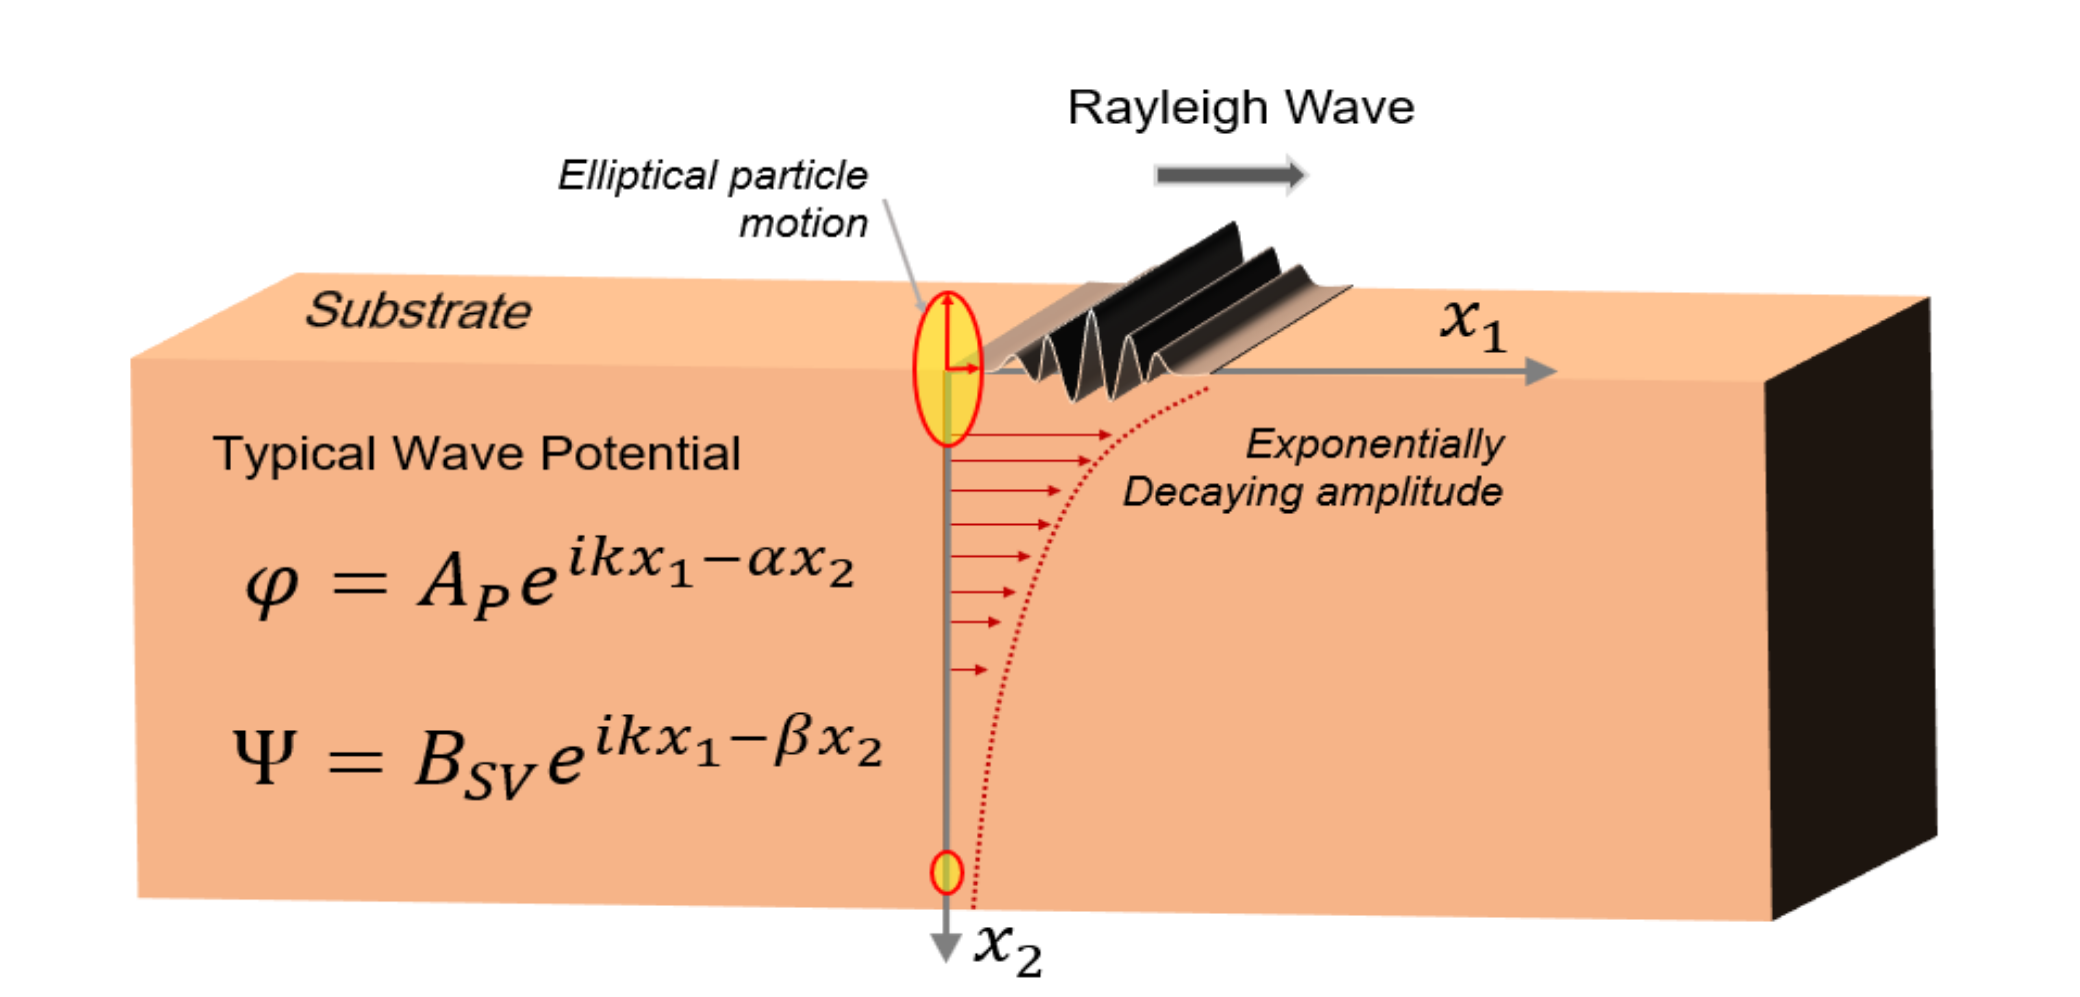
\includegraphics[width=0.8\textwidth]{images/Screenshot-20230208172733-2080x997.png}}
    \caption{Depiction of Rayleigh-Waves propagating through a substrate. \cite{mandalSurfaceAcousticWave2022}}
    \label{fig:rayleigh}
\end{figure}

Other types of SAW waves include \emph{shear horizonal waves} and \emph{Lamb Waves}, however these wave types do not cause the strong vertical displacement which is of interest for the purpose of liquid atomization. From now on the term SAW will be used synonymously for Rayleigh waves.

For most applications, SAW are produced by fixing an \emph{interdigital transducer} (IDT) to a \emph{piezoelectric} substrate. An IDT is a type of electrode strucure consisting of two sets of interleaved metal fingers, which are connected to the opposite poles of a voltage source. Applying an AC current to the IDT produces surface waves by exploiting the piezoelectric properties of the substrate.

A piezoelectric material generates an electrical voltage in response to applied mechanical stress, and conversely generates mechanical displacement in response to applied electrical voltage. 
The piezoelectric effect stems from the relative displacement of oppositely charged ions in a crystal with asymmetrical unit cells causing a displacement of the charge concentration and resulting in a larger electric dipole moment. 
If the dipols in the crystal are aligned, the effect causes the whole crystal to be polarized, creating an electric voltage. 
Since the dipol moments in a crystal are typically only aligned locally in their respective Weiss domains, materials usually need to be poled in order to exhibit strong piezoelectric properties. \cite{liLeadfreePiezoelectricMaterials2021}
All piezoelectric materials also exhibit the reverse effect; applying a electrical field exerts electrostatic force on the dipols which causes displacement of the ions.

\begin{figure}[htbp]
    \centering
    \makebox[\textwidth][c]{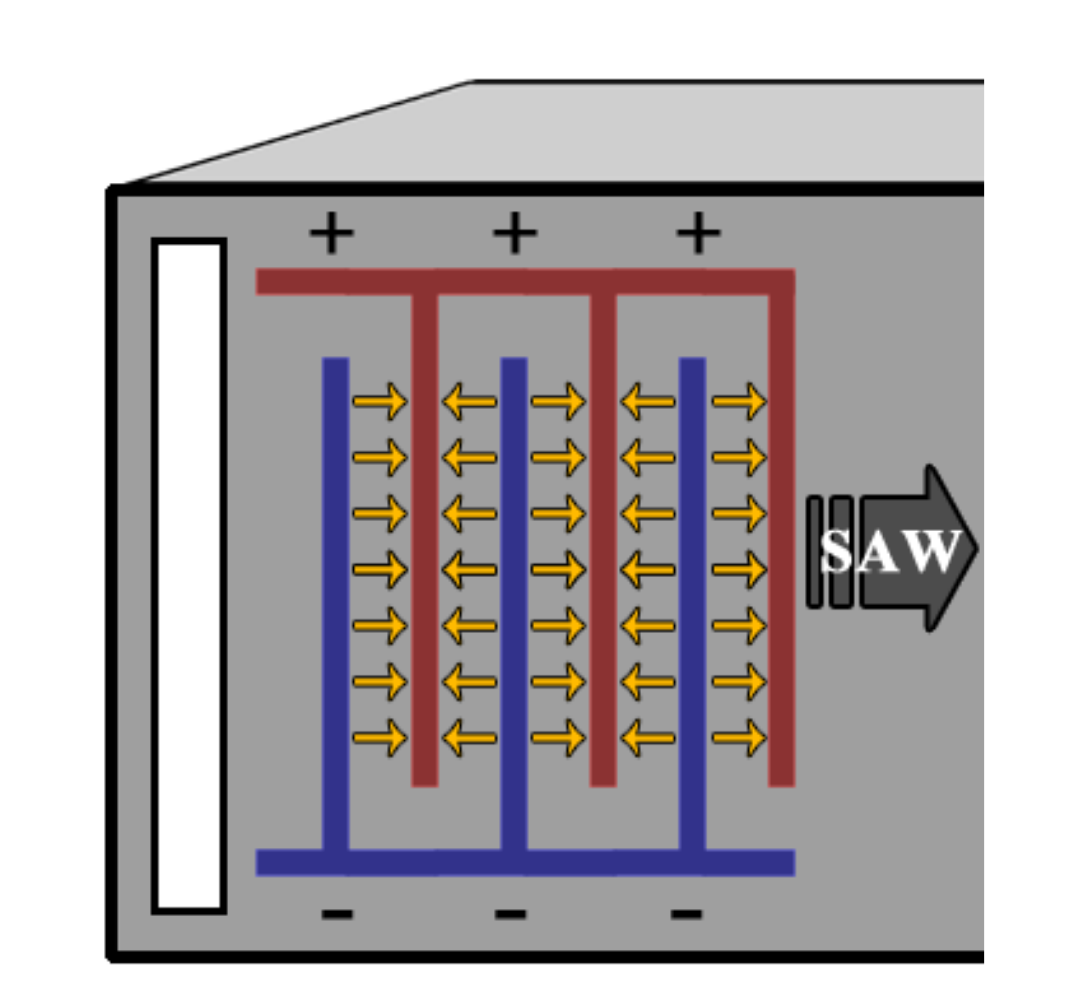
\includegraphics[width=0.4\textwidth]{images/Screenshot-20230208192523-1078x984.png}}
    \caption{The principle of SAW generation in a piezoelectric substrate. A voltage is applied to the two parts of an IDT, which causes mechanical tension in the substrate.}
    \label{fig:idt}
\end{figure}

Since the mechanical force caused by the phenomenon is parallel to the elctrical field, applying AC voltage to the IDT arranged how can be seen in Figure \ref{fig:idt} generates surface waves perpendicular to the direction of the electrodes.

Conversely, the same construction can be used to to pick up vibrations and convert them back to electrical voltage. 
This is the principle commonly used in SAW based sensors, which is only one of many useful applications of SAW technology like filtering in radio frequency technology or compact voltage transformers. 
In the next section the possible application for fluid atomization will be further discussed.
    \section{SAW as a method of fluid atomization}
\label{sec:saw_vapour}

Using SAW technology to produce small scale fluid atomization devices is not a recent idea. 
The concept was already demonstrated by \Citeauthor{kurosawaSurfaceAcousticWave1995}\cite{kurosawaSurfaceAcousticWave1995} in 1995, but mass produced SAW-based atomizers are still not commercially available, likely due to challenges related to the precision engineering required for mass production.

However, because of the many possible applications of low-power, compact fluid atomizers such as inhalation therapy \cite{qiMiniatureInhalationTherapy2009a}, thin film deposition \cite{murochiDepositionThinFilm2007} or nanoparticle synthesis \cite{alvarezRapidGenerationProtein2008}, there is still a substantial interest in improving the technology and optimizing it for production.

Depending on the boundary conditions various acoustofluidic effects can take place during the interaction between SAW and a fluid \cite{winklerSAWbasedFluidAtomization2015a}.
The geometry of the liquid volume has a large on the physical phenomena at play and may result in different atomization regimes, some of which are not entirely understood yet \cite{collinsAtomizationThinWater2012,huangExperimentalResearchSurface2022}.
Describing these highly complex microfluidic phenomena in their entirety is beyond the scope of this work, which is why the following section will focus on the general principle of fluid atomization without going into detail about the governing equations.

When the SAW hits the liquid surface, it is diffracted into the liquid volume at the \emph{Rayleigh angle} $\theta_\text{R} = \sin^{-1}(c_\text{l}/c_\text{SAW})$, which depends on the speed of sound in the liquid $c_\text{l}$ and the propagation speed of the SAW $c_\text{SAW}$ and is $\sim\SI{22}{\degree}$ for water.
The acoustic radiation \emph{leaked} into the liquid causes a longitudinal pressure wave which leads to a bulk recirculation of the liquid known as \emph{acoustic streaming}.

This phenomenon is useful for a variety of applications, such as the mixing of liquids or the transport of particles in a liquid, but is not primarily responsible for the atomization process.
However it has an important influence on the geometry of the liquid volume, which has a significant impact on the droplet formation, as mentioned earlier.

The main driving force behind the atomization process is the capillary waves that form on the liquid surface.
The vertical surface displacement observed for Rayleigh waves is only around \SI{10}{\nano\meter}, however particles are accelerated at around \SI{e7}{\meter/\second\squared}.
If enough power is used, the capillary waves can be amplified to a point where they overcome the surface tension to break and form droplets.

\begin{figure}[htbp]
    \centering
    \makebox[\textwidth][c]{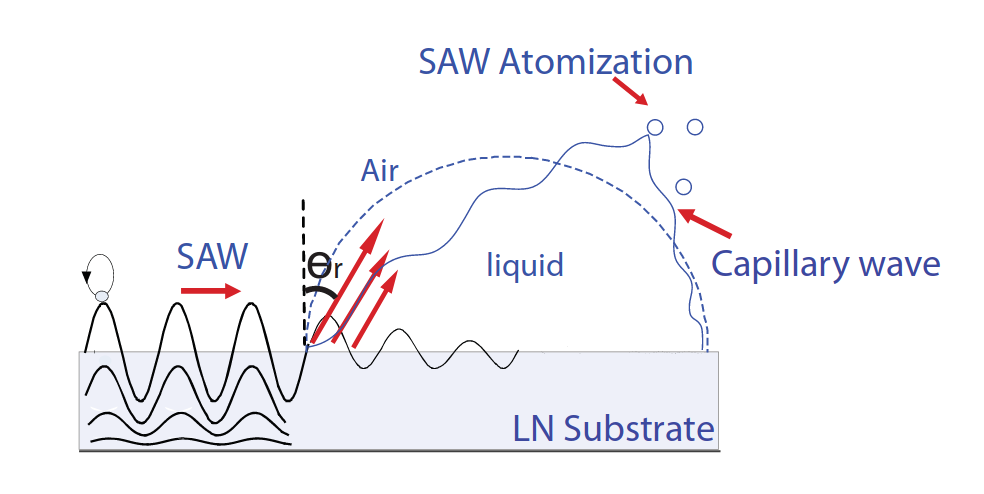
\includegraphics[width=0.7\textwidth]{images/Screenshot-20230211174610-984x494.png}}
    \caption{Schematic depiction of the SAW atomization process. The wave hits the and causes capillary waves on the liquid air interface. \emph{LN} stands for \emph{lithium niobate}, a commonly used piezoelectric material. \cite{aishaqiInvestigationSAWAtomization2009}}
    \label{fig:atomization}
\end{figure}

The exact relationships between the excitation frequency, the capillary wave frequency and the droplet size are not fully understood yet and different models haven been proposed over time.
The main influences in the relationship appear to be the liquid viscosity, the liquid surface tension and the liquid density \cite{aishaqiInvestigationSAWAtomization2009,huangExperimentalResearchSurface2022}.
The latest findings suggest that that the droplet size $D$ is in the same order of magnitude as the wavelength of the capillary waves $\lambda_\text{c}$, which seems to be inversely proportional to the excitation frequency $f$ \cite{collinsAtomizationThinWater2012}.
$$
    D \sim \lambda_\text{c} \sim \frac{1}{f}
$$

Different SAW atomizers differ primarily in how they supply liquid to the atomization area, examples including a \emph{droplet-on-demand} system, where the liquid is supplied by a syringe pump, or a \emph{continuous flow} system, where wetted laboratory paper is placed  on the substrate and the liquid is supplied by a reservoir, with atomization taking place at the meniscus that forms at the edge of the paper \cite{winklerSAWbasedFluidAtomization2015a}.

The method of liquid supply developed at our institute uses a small capillary channel that is mill-cut directly into the substrate, which has direct contact to a liquid reservoir, filling itself using the capillary effect.
This method is very simple and does not require any additional components, which makes it very suitable for mass production.
Ongoing research explores the influence of channel geometry on the atomization process \cite{kapplAkustischInduzierteVernebelung2022}.


    \section{Droplet Measurement Techniques}
\label{sec:measurement_techniques}

For most applications of microparticle aerosols droplet size is a key variable that needs to be controlled precisely to achieve the best results.

For example, in the case of a drug delivery system, the size of the droplet determines the amount of drugs that are absorbed in the lungs, as well as the locations they are deposited in, with smaller droplets reaching more deeply into the lungs, but releasing a smaller amount of drug per unit surface, while larger droplets are more likely to be deposited in the upper airways, but release a larger amount of drug per unit surface area \cite{labirisPulmonaryDrugDelivery2003}.

THerefore, when developing such a system accurate measurement of the droplet size is essential. There are a number of techniques that can be used to measure the size of a droplet, but most of them have some drawbacks or are not suitable for use in this particular application. 
This section gives an overview on the most common techniques as well as our method.

\paragraph{Laser diffraction techniques} make use of the fact that the diffraction angle of light passing a sphere is proportional to the diameter of the sphere, with large particles scattering the light at smaller angles and smaller particles scattering the light at larger angles, according to \emph{Mie theory} for electromagnetic wave scattering \cite{drakeMieScattering1985,wriedtMieTheoryReview2012}.

Devices pass a laser beam through the vapour and record the angular scattering intensity, which is then analyzed to calculate the size of the particles. 

Theoretically, laser diffraction techniques are very accurate and able to measure particles as small as \SI{0.1}{\micro\meter} and have been used to measure SAW atomized particle distributions previously. 
However, a company which is in a cooperative relationship with our institute for the purpose of researching SAW atomization has reported inconsistencies in their use of a commercially available device, which is why we have chosen to investigate other techniques.
Another reason for choosing other techniques is the potentially prohibitive pricing of the laser diffraction devices in this stage of the research.

\paragraph{Phase Doppler Particle Analysis (PDPA)} uses two laser beams that cross each other in a volume with an ellipsoidal cross section in which an interference pattern between the lasers is produced, forming fringes of differing light intensity \cite{hollPARTICLEDEPOSITIONVELOCITIES}.
When a particle passes through the volume, this fringe pattern is scattered, which produces pulses of light called \emph{doppler bursts} that can be picked up by two or more well placed photo detectors.
Information about the particle can be extracted from the phase difference of the doppler bursts picked up by the different detectors.

PDPA is a very accurate technique, but requires very large and specialized equipment, with commercial devices facing similar drawbacks to laser diffraction devices in terms of price and size.

It is also known to produce inaccurate readings for inhomogeneous particles or other disturbances in the measurement environment, which requires a more complicated set up \cite{sijsDropSizeMeasurement2021}.

\paragraph{Image Analysis} 
The technique used during research up until this point employs a more pragmatic approach. A high speed camera in combination with a microscope objective lens and a parallel light source is used to record images of the aerosolized particles as they are being produced. The images were then analyzed manually one by one to determine the size of the particles. While being very flexible and easy to calibrate, this is an extremely tedious and time consuming process, since each droplet has to be measured individually.

This is the aspect of the research that this thesis aims to improve upon by utilizing machine learning techniques to automate the process of droplet identification and subsequent size measurement.

Using this kind of image analysis method is not unprecedented, as \Citeauthor{sijsDropSizeMeasurement2021}\cite{sijsDropSizeMeasurement2021} have demonstrated a similar approach in 2021, where they use image processing techniques to identify and measure droplets in image data. 
However, they do not disclose the details of their image processing pipeline, making it unclear if they employ machine learning models for this purpose.
While the idea behind their approach seems to be similar, \Citeauthor{sijsDropSizeMeasurement2021} report a minimum droplet size of \SI{150}{\micro\meter} for their technique, which is one to two orders of magnitudes larger than our expected droplet size of \SIrange{1}{30}{\micro\meter}.
As a result, their images seem to have much less noise and uneven lighting conditions, which makes droplet identification easier.
The method used in this thesis is therefore more applicable to the kind of images that we are working with, but could be used for the same purpose when measuring larger droplets.



    \newpage
    \chapter{Theory from the perspective of Computer Science}
    \label{sec:theory_compsci}
    As stated in the Introduction, the goal of this thesis is to use a neural network to identify the droplets in the captured image data. The problem lies in the domain of \emph{segmantic pixel level image segmentation} and the employed network is a kind of \emph{(Deep-)Convolutional Neural Network} (DCNN). In the following section, a brief overview of the basics of neural networks, how they work in general and how they can be adapted to a certain task is given. 

\subsection{Basics and buidling blocks of neural networks}
\label{sec:building_blocks}

The idea of artificial neural networks came long before the capability to employ them as a tool and stems from research in trying to model how biological neurons function. Biological nerve cells receive signals from several other neurons and send a signal on their own based on the strength of their inputs. Translating this behaviour to a mathematical model brings us to the \emph{single layer perceptron}.

\paragraph*{Perceptron}

\begin{figure}[htbp]
    \makebox[\textwidth][c]{
    \tikzset{basic/.style={draw,fill=blue!20,text width=1em,text badly centered}} 
    \tikzset{input/.style={basic,circle}} 
    \tikzset{weights/.style={basic,rectangle}}
    \tikzset{functions/.style={basic,circle,fill=blue!10}}

    \begin{tikzpicture} 
        \node[functions] (center) {}; 
        \node[below of=center,font=\scriptsize] {Activation function}; 
        \draw[thick] (0.5em, 0.5em) -- (0,0.5em) -- (0,-0.5em) -- (-0.5em,-0.5em); 
        \draw (0em,0.75em) -- (0em,-0.75em); 
        \draw (0.75em,0em) -- (-0.75em,0em); 
        \node[right of=center](right) {}; 
            \path[draw,->] (center) -- (right); 
        \node[functions,left=3em of center] (left) {$\sum$}; 
            \path[draw,->] (left) -- (center); 
        \node[weights, left=3em of left] (2) {$w_2$} -- (2) node[input,left of=2] (l2) {$x_2$};
            \path[draw,->] (l2) -- (2); 
            \path[draw,->] (2) -- (left); 
        \node[below of=2] (dots) {$\vdots$} -- (dots) node[left of=dots] (ldots) {$\vdots$};
        \node[weights,below of=dots] (n) {$w_n$} -- (n) node[input,left of=n] (ln)
    {$x_n$}; \path[draw,->] (ln) -- (n); \path[draw,->] (n) -- (left);
        \node[weights,above of=2] (1) {$w_1$} -- (1) node[input,left of=1] (l1)
    {$x_1$}; \path[draw,->] (l1) -- (1); \path[draw,->] (1) -- (left);
        \node[weights,above of=1] (0) {$w_0$} -- (0) node[input,left of=0] (l0) {$1$}; 
            \path[draw,->] (l0) -- (0); 
            \path[draw,->] (0) -- (left); 
        \node[below of=ln,font=\scriptsize] {inputs}; 
        \node[below of=n,font=\scriptsize]{weights}; 
    \end{tikzpicture}
    }
    \caption{Displayed is a schmematic of the single layer perceptron. $x_i$ are the inputs that get multiplied by the weights $w_i$. $w_0$ is also called the \emph{bias}. The product of weights and inputs is then summed up and passed to an activation function that computes the output of the perceptron.}
    \label{fig:perceptron}
\end{figure}

The perceptron displayed in \ref*{fig:perceptron} computes its output like
$$
    o = f\left(w_o + \sum_{i} w_i x_i\right)
$$
where $f$ is the activation function, which is some derivable nonlinear function. State of the art networks use mostly the \emph{Rectified Linear Unit} (ReLU) as their activation function, which has proven to be preferable to its predecessor, the sigmoid function, and is computed as such:
$$
    \text{ReLU}(x) = \begin{cases}
        x, &x>0\\
        0, &\text{else}
    \end{cases}
$$

Naturally, modern networks contain much more than one neuron and instead contain many such nodes, that are interconnected with each other. 
These neurons are typically organized in \emph{layers} and form, in the case of feedforward networks, an acyclic directed graph, where neurons of one layer are only connected to the neurons in layers further down the pipeline. Often the layers between output layer and input layer are called \emph{hidden layers}, since the intermediate representation of the input data they compute is not immediately of interest.

While a single neuron doesn't have the capability to solve complex problems, it has been show that a network with as little as one fully connected hidden layer (all neurons of the previus layer output to all neurons of the following layer) can function as a \emph{universal approximator} for functions between two Euclidean spaces\cite{hornikMultilayerFeedforwardNetworks1989} or indeed any $L^p$-Space\cite{parkMinimumWidthUniversal2020}. This means if there is a mathematical correlation between our desired input and output, so long as both can be represented in these spaces, we can find a neural network that approximates this correlation very well.

While this is an extraordinary finding, modern neural networks often place much more emphasis on the number of layers (depth) than the number of neurons in one layer (width) of a network, hence the terms \emph{deep learning} or \emph{deep neural networks}. However, the size of a networks parameters and with that needs for computational power climbs fast when using many fully connected layers. One tool that enables the use of very deep networks is the \emph{convolutional layer}.

\paragraph*{Convolutions and convolutional neural networks}

Similarly to a discrete 2d convolution in mathematics, a convolutional layer in a neural networks moves over the input space with a comparatively (to input dimensions) smaller kernel and computes the output by multiplying the weights stored in the kernel with the corresponding input values.

\begin{figure}[htbp]
    \makebox[\textwidth][c]{
        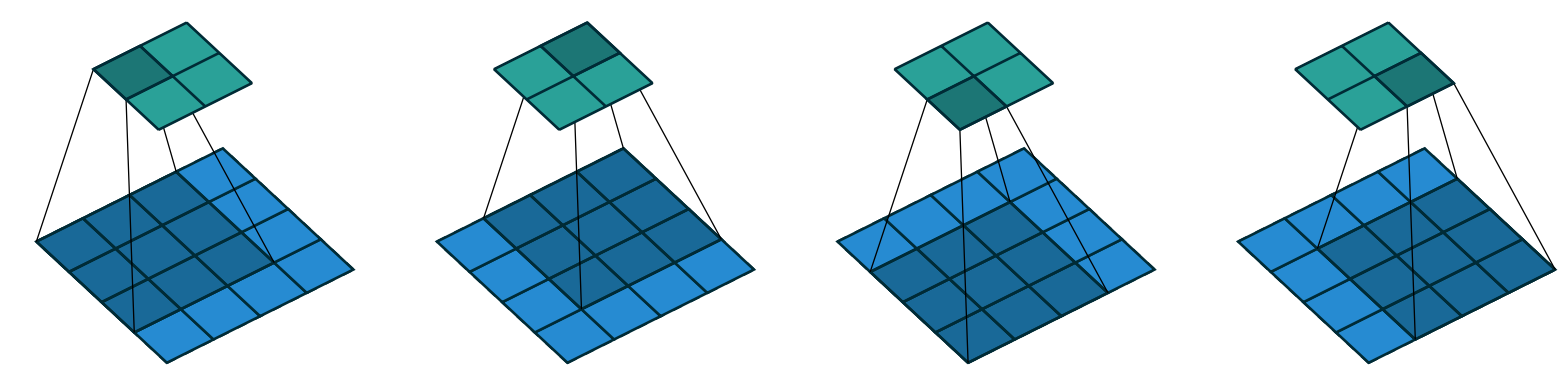
\includegraphics[width=\textwidth]{images/att_00028.png}
    }
    \caption{Depiction of how a convolution computes its outputs. A $4\times 4$ input convolved with a $3\times 3$ kernel produces a $2\times 2$ output. Since no padding is used this constitues a valid convolution. \href{https://fastai.github.io/fastbook2e/images/att_00028.png}{Image Source}}
    \label{fig:convolution}
\end{figure}

The example seen in Figure \ref*{fig:convolution} shows only one channel and a procedure that employs no padding, leaving the output smaller than the input (called a valid convolution). Other than valid convolutions, padding the input by $\lfloor\frac{k}{2}\rfloor$ or $k - 1$, where $k$ is the size of the kernel, leaves us with a \emph{same} (same size as input) or \emph{full} (larger than input) convolution. Additionally, in reality inputs to a layer often have many channels and the layer should be able to produce an arbitrary amount of output channels. In this case there exists a kernel $K_{\text{in}, \text{out}}$ for each combination of input channels $C_\text{in}$ and output channels $C_{\text{out}}$ whose convolution results are then added up for each output channel, so that
$$
    \text{out}_j = \sum_{k=1}^{C_\text{in}} K_{k,j} * \text{input}_k
$$
where $*$ is the convolution operation. There are other approaches to handle multi channel scenarios, but this is the simplest one and the one employed in the thesis. 

Using a convolution layer has several advantages over using fully connected layers. First of all is a reduction in \emph{learnable parameters} (see \ref*{sec:training}) which reduces computational resources required and thereby speeds up training. Secondly it introduces the inductive bias that positionally close data points are correlated and relevant to each other to the model, which is reasonable especially in tasks concerning computer vision. 

Imagine having a model that tries to detect circles in an image. It makes sense to assume that features which make up a circle are positionally close to each other. Convolutions are also translationally invariant, which in the same example means that for two identical circles at different locations in the input, the identical output is produced at their corresponing position, which is not the case for fully connected layers, where very different weights might me learned for different positions in the picture if data is insufficiently random.

Many architectures in the computer vision field now purely employ convolutional layers (\emph{fully convolutional neural networks}) or use very few fully connected layers only to compute the final output of the network at the end. 

There are additional constructs that can be used in neural networks, such as \emph{pooling} layers, which also move a kernel over the input like a convolution, but instead take the average or maximum of the covered elements as their output. As such, the pooling layer contains no variable parameters. They are generally used to reduce the dimensions of the feature map to further speed up training time and make the model more stable by promoting invariance to small perturbations in the input.
    \section{Semantic Image Segmentation}
\label{sec:imseg}

With the knowledge of how neural networks perform their computation in general we need to think about how a specific task can be accomplished by them.
To do this we need to find a specialized representation of the problem which networks can be applied to.

There are several common types of problems within computer vision that have different kinds of encodings for their solution space. As stated in the introduction, the task which this thesis is trying to solve lies in the category of \emph{Instance Segmentation}, but can be accomplished by instead doing \emph{Semantic Image Segmentation}.
For this task the network input is an image and the network is supposed to assign each pixel one of a predetermined set of \emph{classes} to which the pixel belongs to. For example in the case of the \emph{Cityscapes Dataset}\cite{cordtsCityscapesDatasetSemantic2016a}, the data consists of images of inner city traffic situations from the perspective of a car, and the classes are subjects like \emph{car}, \emph{road}, \emph{person}, \emph{building} etc.

\begin{figure}[htbp]
    \centering
    \begin{tabular}{ll}
        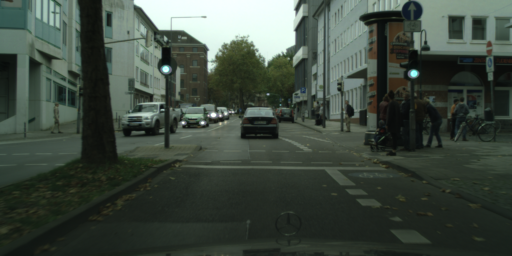
\includegraphics[width=0.45\textwidth]{images/aachen_000029_000019_leftImg8bit.png}
        &
        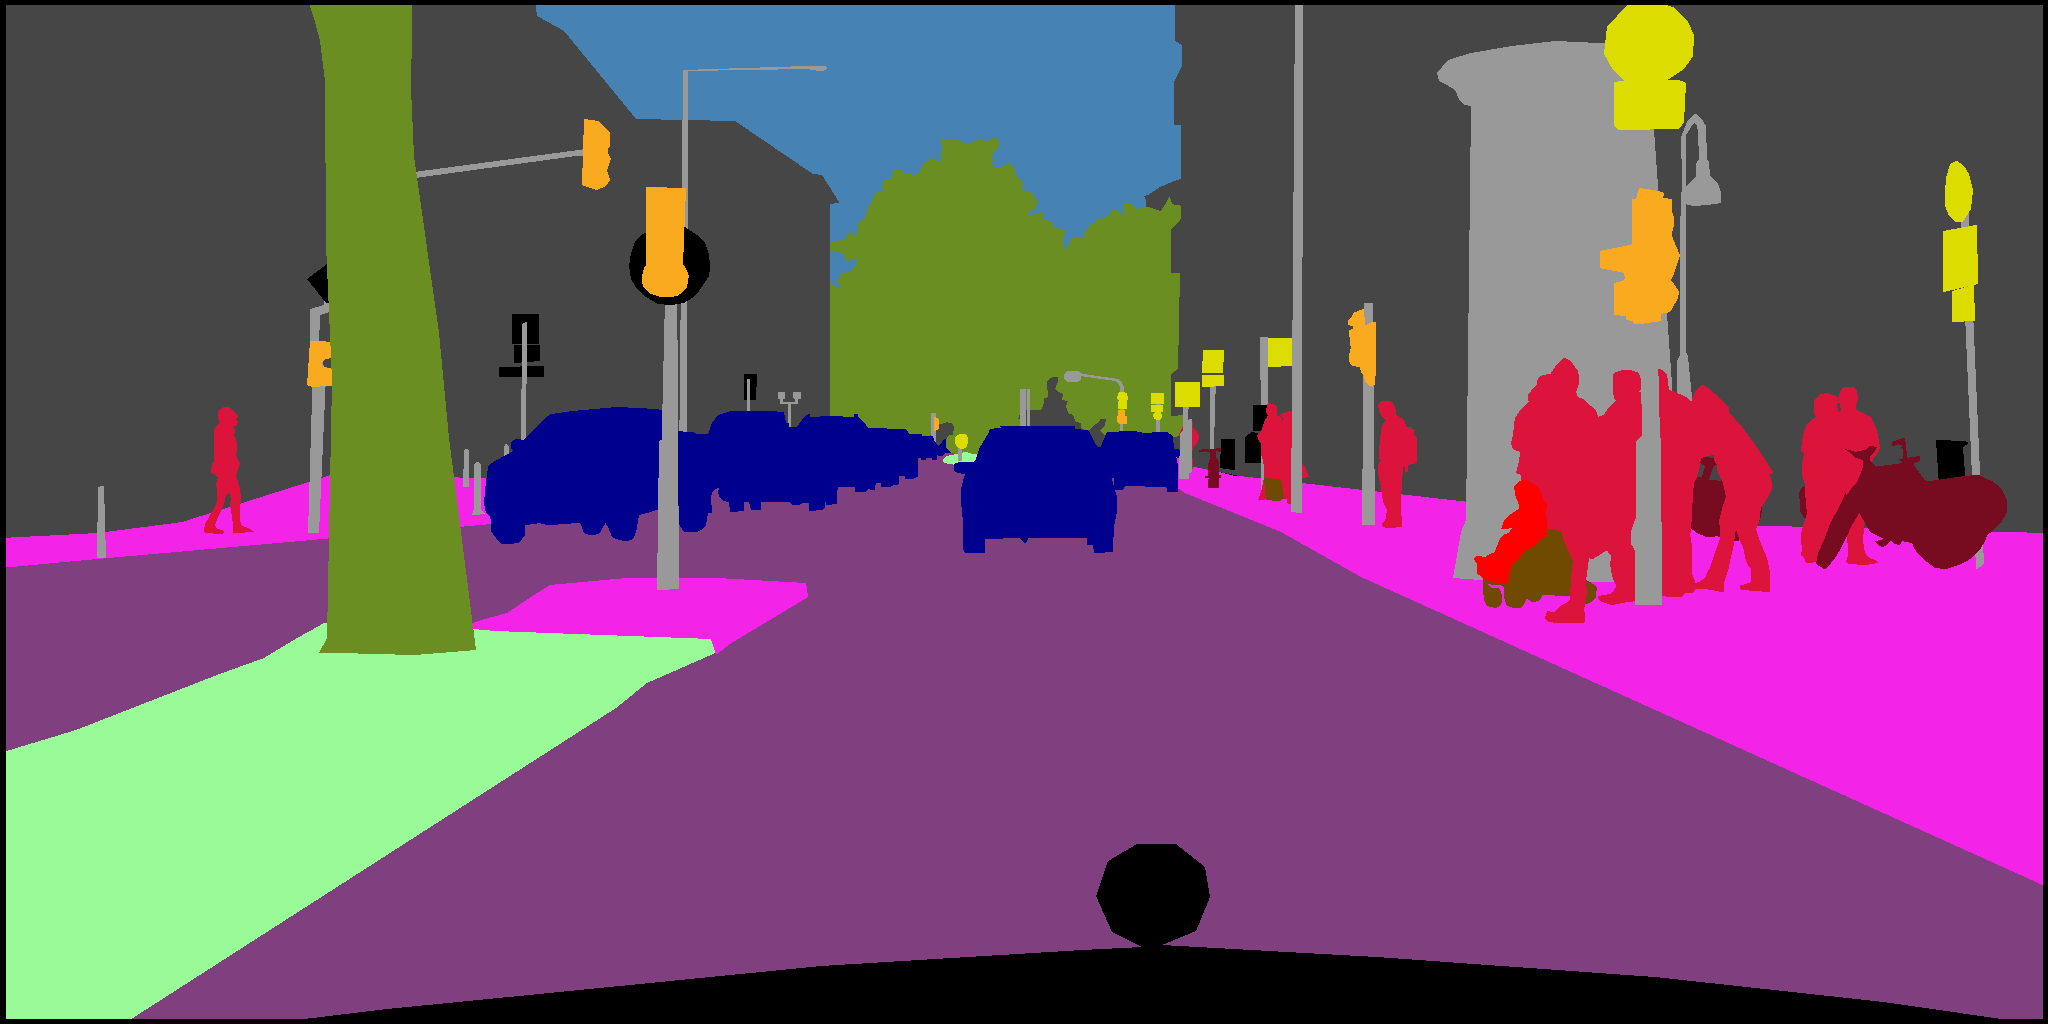
\includegraphics[width=0.45\textwidth]{images/aachen_000029_000019_gtFine_color.png}
    \end{tabular}
    \caption{A sample from the dataset \emph{Cityscapes}. On the left is the image that acts as an input for the network and on the right is the corresponding ground truth label mask showing different classes in different colors. \cite{cordtsCityscapesDatasetSemantic2016a}}
    \label{fig:cityscapes_smpl}
\end{figure}

A model for this task would now output a map $O\in\mathbf{R}^{C\times M\times N}$ with the same spatial dimensions as the image and a number of channels $C$ equivalent to the number of possible classes. Each output pixel consists of a vector $\mathbf{x}\in \mathbb{R}^C$ where each entry $x_i$ corresponds to how much the network thinks the pixel belongs to class $i$. The channel with the highest value is the class the network has classified the pixel as.

These outputs can now be normalized to probabilities by applying the \emph{softmax} function to them or converted to a segmentation mask by using the \emph{argmax} function.

To evaluate how well a network performs on the segmentation task, the \emph{Intersection over Union} (IoU) for each class is computed. For the set $A$ of pixels labeled as a certain class by the network and the set $B$ of pixels which are part of that class in the ground truth the IoU is defined as
$$
    \text{IoU} = \frac{\left|A\cap B \,\right|}{\left|A\cup B \,\right|}\quad .
$$
This metric is very informative to look at per class when trying to figure out specific strengths and weaknesses of the model, but typically the mean over all classes (mIoU) is used to evaluate the model as a whole.

A big challenge in developing machine learning solutions for this kind of task is its demand for varied data to train models on. High quality annotated data is very time and cost consuming to produce. 
For example according to the Cityscapes team, one annotated image such as seen in Figure \ref{fig:cityscapes_smpl} took \SI{90}{min} to create. 
Further in this thesis techniques to mitigate this problem and achieve good results on a small set of annotated data will be discussed.

    \section{Training neural networks}
\label{sec:training}

As mentioned previously neural networks with appropriate weights can be used to approximate any mathematical mapping between two Euclidean spaces (and more), but which weights are appropriate is not at all apparent for any nontrivial task. 
Similarly to how humans don't immediately perform at their potential best at a new task, but can train the brain to improve at solving a particular problem by strengthening the corresponding nervous pathways through repeated exercise, a neural network can \emph{learn} the correct weights for a task during \emph{neural network training}.

Training a neural network requires annotated data for a problem, where the ground truth for the problem at hand is known and encoded in a way that is compatible with the output format of the neural network. 
Keeping in line with the topic of this thesis, for a pixel level semantic segmentation task, this would be in the form of segmentation masks where each pixel has the id of the correct class as its value. 

Training happens in several steps. First, a sample from the training data is taken and the model, typically initialized with (semi-) random weights, computes its prediction for the problem (a segmentation mask). Then, a \emph{loss function} is applied to measure a distance between the prediction and the ground truth in the solution space. 
There are several functions which can be used as a loss function for one particular problem which may or may not perform better than others in expressing how wrong the model was with its prediction. 
Next, the gradient of the loss with regards to each learnable parameter is computed by using the chain rule for derivatives to propagate the error backwards through the network (\emph{backpropagation}). 
The parameters are then very slightly adjusted to reduce that error. 
There are several different rules for updating the weights with this gradient in each step, but widely used procedures include \emph{stochastic gradient descent (SGD)} and \emph{adam} \cite{kingmaAdamMethodStochastic2017}. 

There are several parameters that influence the progress of the training or even how the model operates, but aren't learnable parameters like the weights of the model. 
These parameters are called \emph{hyperparameters}. This includes the \emph{learning rate} which influences how much the parameters get updated in each step, but also things like the kernel size of a convolutional layer. 
Most of the time, samples aren't processed one by one, but stacked up in \emph{batches}, whose size (the \emph{batch size}) constitute another important hyperparameter. 
Processing multiple samples at once can be more efficient and also make the training process more stable by presenting more varied data to the network during each optimization step. However, batch size is limited by the size of the training samples in relation to the memory of the hardware used, so it can't be made arbitrarily large. 

Which hyperparameter values are used during training can have a huge impact performance, so finding optimal hyperparameters is vital when developing a model. 
The appropriate hyperparameters depend a lot on the training data and model architecture and are largely determined through trial and error. 
There are systematic approaches to hyperparameter tuning, but these are often very computationally expensive, since they perform a lot of trial runs. 
For simpler problems it is often enough to perform the search manually, by starting at values which are known to be in the correct order of magnitude for similar problems and then make informed adjustments based on the results of fewer trial runs. 

Another important part of model training is \emph{data augmentation}, which means to apply random perturbations to the inputs or even the model itself (in the case of \emph{dropouts}) during training to prevent the model from \emph{overfitting}. 
This refers to the model \emph{memorizing} the training data instead of learning the concept of the problem, leading to high performance on the training data at the cost of worse performance on unseen data, which is undesirable in most cases. 
The noise applied by augmentation reduces the likelihood of this happening and generally improves model performance. 
Since the augmentations are random, they functionally produce additional samples, which can help especially in cases with little training data. 
Some typical augmentations for computer vision tasks include \emph{random horizontal/vertical flipping}, \emph{scaling and resizing} or \emph{applying gaussian noise}. 

    \chapter{Architectures}
    \label{sec:architectures}
    When approaching a problem with a machine learning solution in mind, the first decision one has to deliberate on is the choice of network architecture used. 

In the case of neural networks, the word \emph{architecture} means which kind of layers are connected to each other in what order to produce the output of the network.

The landscape of machine learning architectures has become incredibly diverse, with improvements being made constantly.
With some architectures being better suited for certain problems or priorities, which architecture one chooses has a significant impact on the results.

In this section, an overview over the architectures used in the thesis and their main ideas will be given.
    \section{The U-Net}

The \emph{U-Net} is a network achitecture first proposed by \Citeauthor{ronnebergerUNetConvolutionalNetworks2015} in 2015 for application in biomedical segmentation tasks, for example segmenting cell borders in microscopic images of HeLa cells. 
The challenges the authors were facing at the time are similar to the ones in this thesis, where training data for biomedical segmentation tasks was scarce, which is why the U-Net was makes sense as a starting point for the problem of droplet segmentation.

It is a fully convolutional network, which were on the rise to surpass older state of the art neural networks for classification tasks at the time. 
The network employs an \emph{encoder-decoder} structure, meaning the architecture consists of a contracting path and a expanding path, the \emph{encoder} and \emph{decoder} respectively, as seen in Figure \ref{fig:unet}.

\begin{figure}[htbp]
    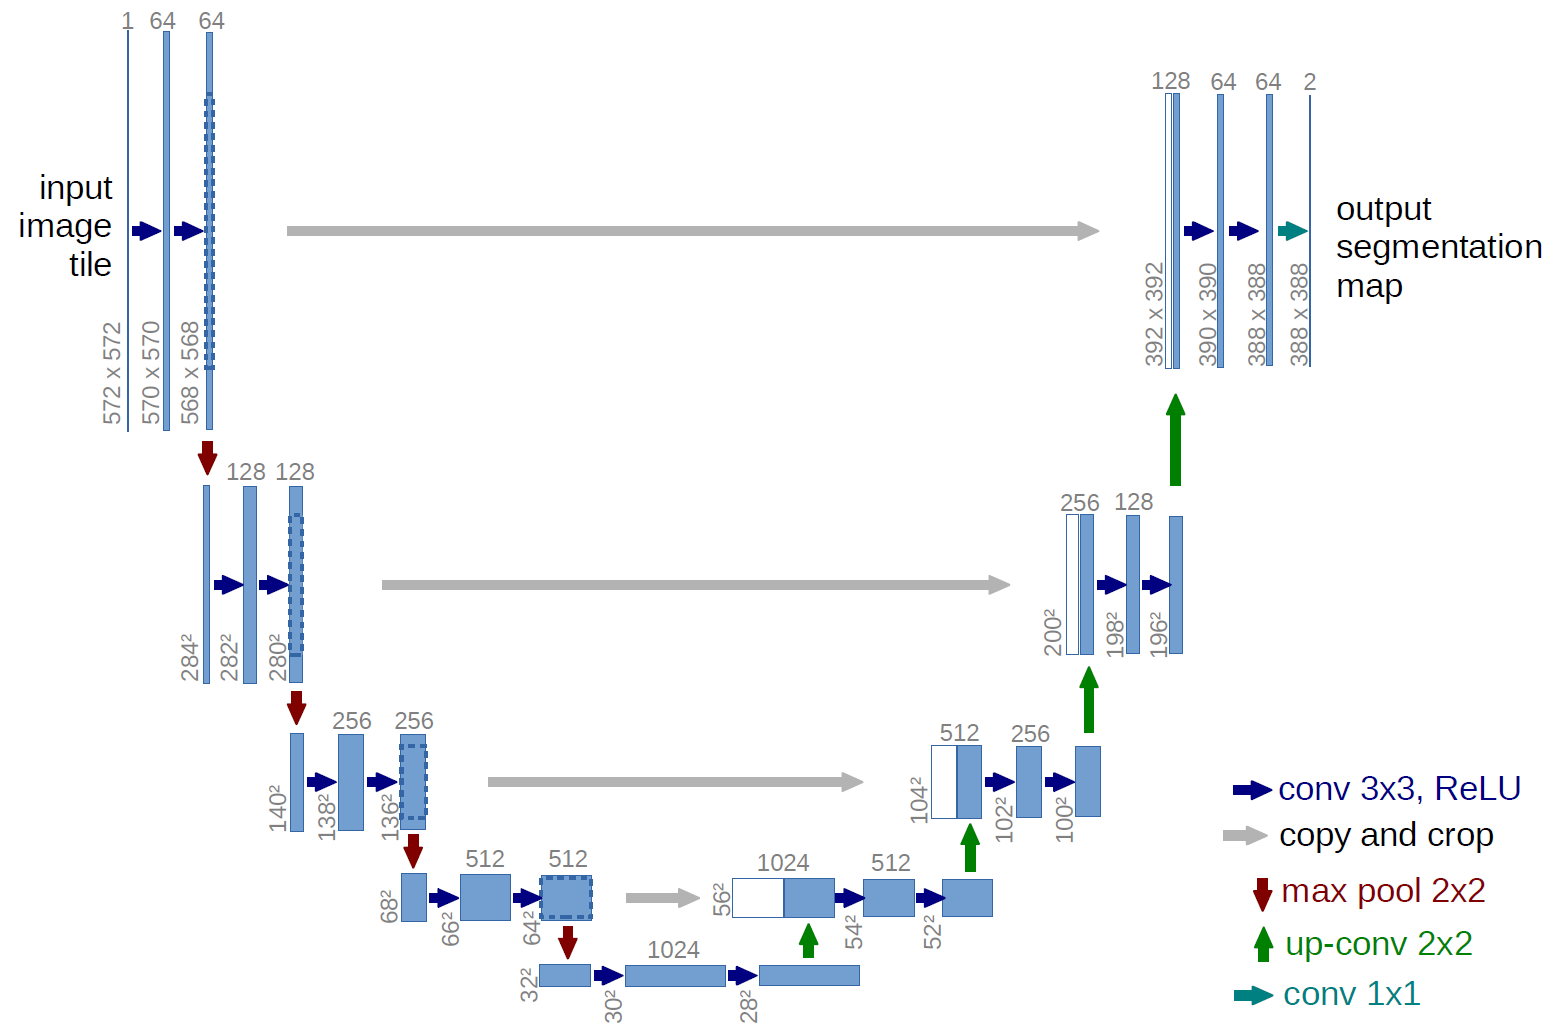
\includegraphics[width=\textwidth]{images/unet.png}
    \caption{The original U-Net architecture proposed in \cite{ronnebergerUNetConvolutionalNetworks2015}, for an example of a $572\times 572$ input, with the number of channels of the layer written above the blue boxes representing the feature map after each layer passthrough. The legend shows which operation was used between each feature map.}
    \label{fig:unet}
\end{figure}

The encoder path computes a number of features at four different spatial input sizes with two $3\times 3$ convolutions followed by a ReLu, which are then downsampled by a $2\times 2$ max-pooling layer. 
With each of these blocks, the spatial resolution is halfed along each axis, while the number of feature channels is doubled.

The features output by each block depend on different sized regions of the initial input. 

The values of blocks with high spatial resolution consider only small patches in the input image, while a lot of pixels influence each value for the lower blocks. 
The large \emph{perceptive field} of the lower blocks allow for rich contextual information to be encoded in their feature maps.

In a classification problem, such contracing networks would be used by feeding the highly dense information of the last encoder block to a few fully connected layers which make the final classification decision. 
In this case, since a classification for each pixel is needed, the encoded information must now be scaled back up to the desired resolution.

The decoder path is symmetrical to the encoder path, halving the number of feature channels in each block and upsampling the spatial resolution by using $2\times 2$ \emph{transposed convolutions}, which act like a backwards pass through a normal convolution.
After the last upsampling block a final $1\times 1$ convolution is used to decide the final class for each pixel.

However, as is, this structure has a key flaw when it comes to creating segmentation masks. While it is feasable to deduce general locations of objects from the highly contextual encoder features, it is difficult to infer their exact boundaries, because the spatial resolution has been compressed so much. 

This is where another key aspect of the U-Net architecture comes in. 
By concatenating the outputs of each encoder block to the input of their respective decoder block, we allow the decoder to not only utlize the context information provided by the last enocoder layers, but also the very localized features of the high resolution blocks.

This combination allows the U-Net to predict the correct classes along with their precise spatial location.

The U-Net outperformed its predecessors by a large margin and has since been developed further. Its concepts still serve as the basis for popular segmentation networks.\\

One way in which the original U-Net architecture is often modified, is using more sophisticated models for the encoder module, which is the approach taken in this thesis. 
Obtaining better features has proven itself to lead to better overall results, so investing more capability in the encoder structure is often a good idea. 

This also comes with the added benefit that pretrained weights for common feature extractors like the \emph{ResNet} (more in \ref{sec:resnet}) are readily available. 
    \section{The ResNet}
\label{sec:resnet}

The \emph{Residual Network (ResNet)} is a deep neural network architecture first introduced by \Citeauthor{heDeepResidualLearning2015}\cite{heDeepResidualLearning2015} in 2015, which addresses the seemingly paradoxical circumstance that adding more layers to a deep neural network would degrade its performance compared to a shallower network, even though the solution space of the shallower model is a subspace of its deeper counterpart. 

Working from the idea that adding more layers to a network should not produce a higher error, since the additional layers could potentially just learn identity mappings, the authors surmised that the problem lied with the difficulty for the optimization process to learn the underlying desired mapping for a set of layers if the ideal mapping is closer to an identity mapping than a zero mapping.

The solution to this, proposed by ResNet, is to utilize residual connections between the input and output of a layer group, by directly adding the input to the output. 
Instead of having to learn the desired output mapping $\mathcal{H}(x)$, the layers now have to fit the residual mapping $\mathcal{F}(x) := \mathcal{H}(x) - x$, which the authors argue is easier for the optimizer to do.

\begin{figure}[htbp]
    \makebox[\textwidth][c]{
        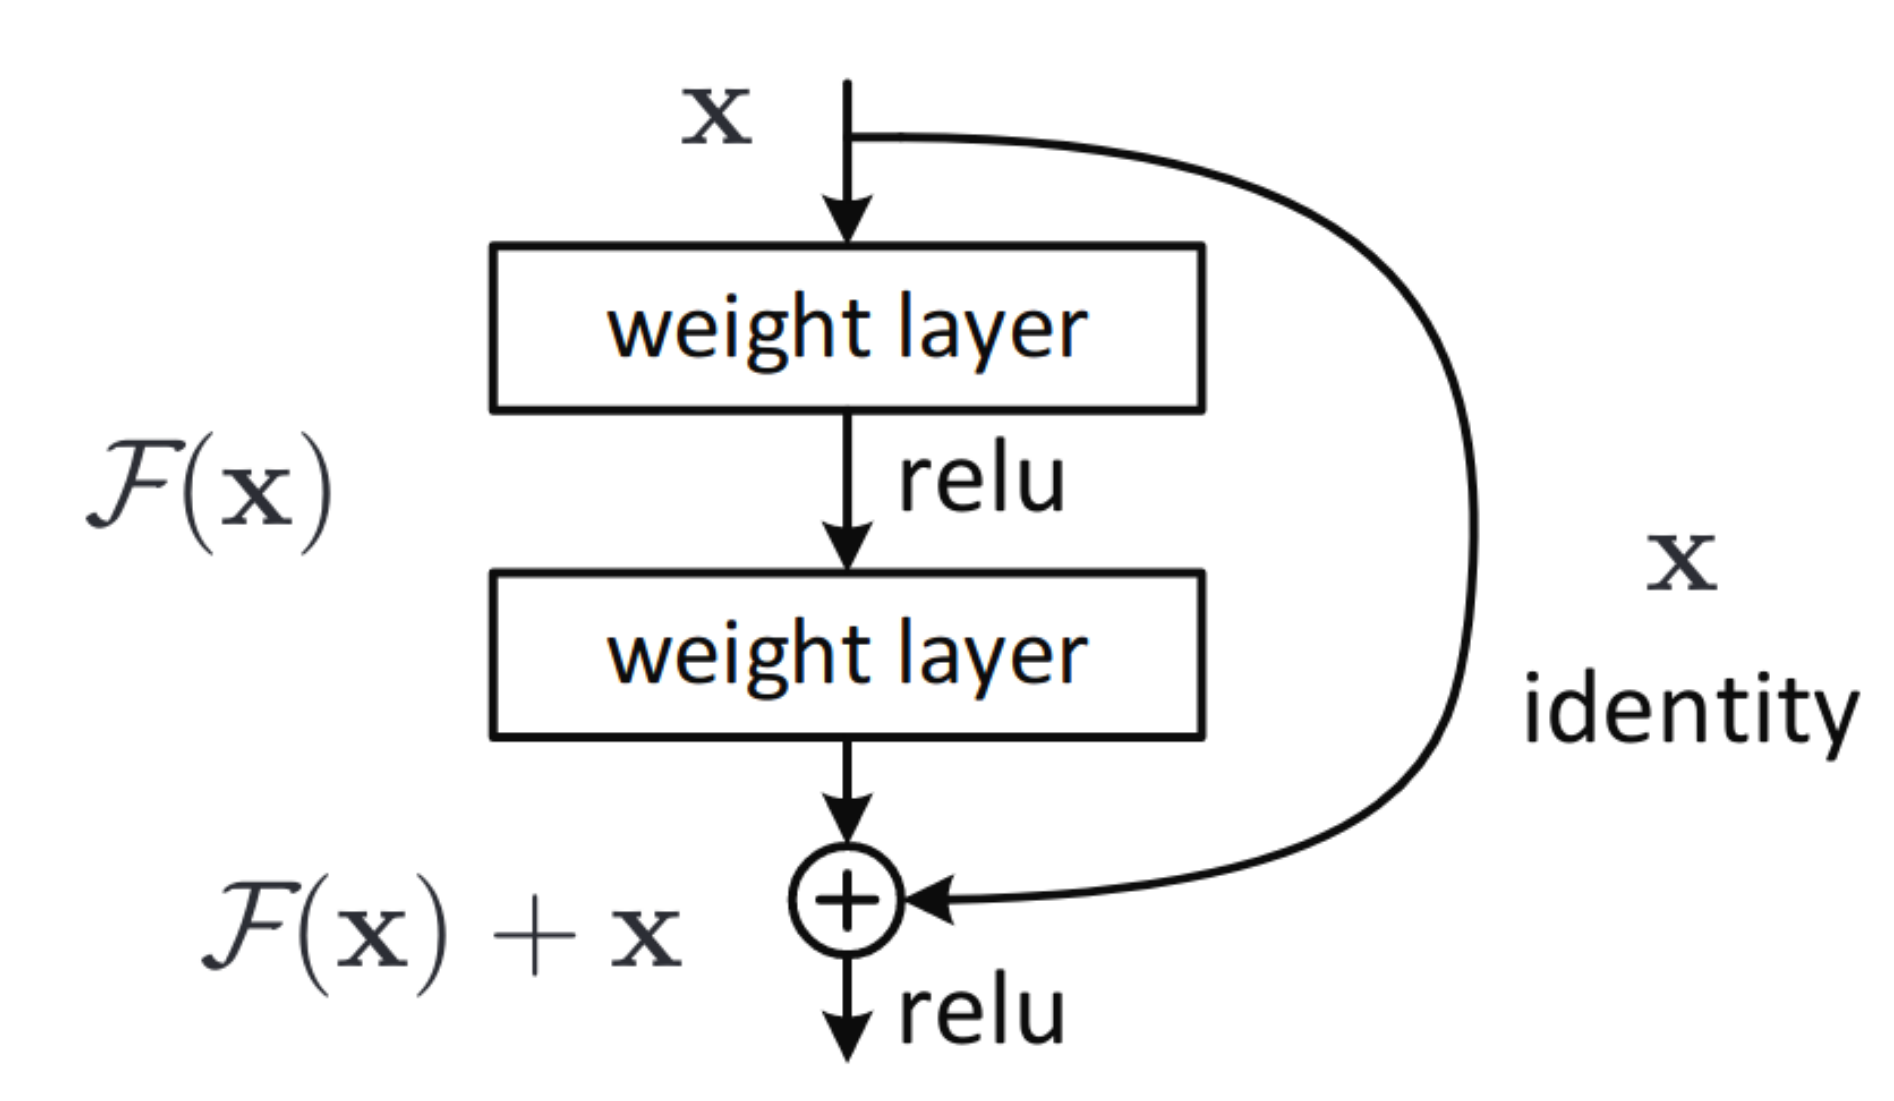
\includegraphics[width=0.4\textwidth]{images/Screenshot-20230207134546-1894x1101.png}
    }
    \caption{A depiction of a \emph{residual block} employed in the ResNet network architecture. The input of a group consisting of several layers is added directly to the output. The weighted layers can be linear layers but in practice, mostly convolutional layers are used. The blocks also consist of 3 layers the majority of the time. Image taken from \cite{heDeepResidualLearning2015}}
    \label{fig:resblock}
\end{figure}

Employing these \emph{residual blocks}, the convergence rate of the network is significantly improved, without adding any computational complexity. 
This enables the use of very deep networks, gaining substantial accuracy from the added layers.

Apart from the residual connections, the ResNet still follows a typical encoder architecture, with each block reducing spatial resolution, while increasing the number of feature channels.
There are several versions of the ResNet architecture, differing mainly by the number of layers used. 
\Citeauthor{heDeepResidualLearning2015} looks at networks with up to 152 layers (ResNet152), but deeper networks have been explored. 

Since the residual connection allow the network to propagate information from the shallower layers to the deeper layers more easily, it may also combat the problem of vanishing/exploding gradients, which were a challenge for increasingly deep models at the time, however the authors argue that this was already sufficiently addressed by regularization techniques such a \emph{Batch Normalization}. \cite{ioffeBatchNormalizationAccelerating2015}

ResNet was able to significantly outperform its state-the-art predecessors at the task of image classification and is widely used today, often as part of a larger model ensemble.

In this thesis, \emph{ResNet34 D} is used in most experiments, which makes several minor improvements over the regular ResNet.
This includes employing an average pooling layer before the strided $1\times 1$ convolution present in the identity path of each downsampling block to include all datapoints, switching the stride of convolutions in the residual path for the same reason and replacing the $7\times 7$ initial downsampling convolution with three $3\times 3$ convolutions.
These modifications see an improvement in classification error while only increasing computational cost slightly. \cite{heBagTricksImage2018} 

\begin{figure}[htbp]
    \makebox[\textwidth][c]{
        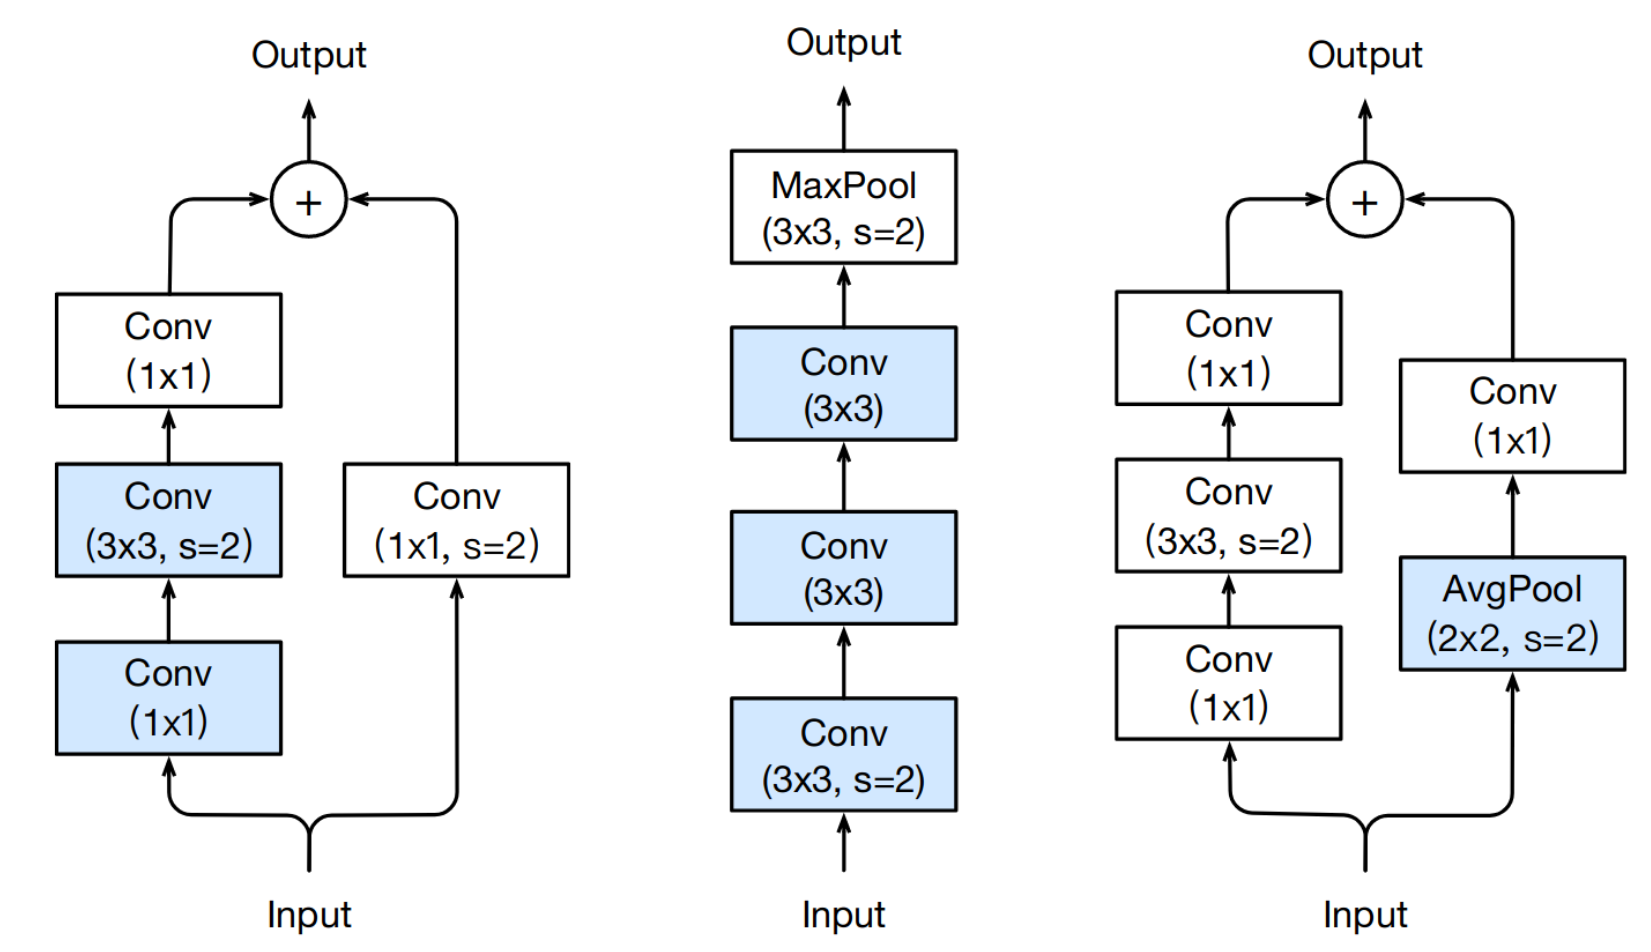
\includegraphics[width=0.9\textwidth]{images/Screenshot-20230207145624-1651x952.png}
    }
    \caption{Illustration of the three improvements made by ResNet34 D, with the blue boxes representing the changes made. Left depicts the change made to the residual path of the downsampling block, middle illustrates the changes made to the initial block of the network and right explains the changes to the identity path. $s$ represents the stride of the operations, with it being one if ommited. Image taken from \cite{heBagTricksImage2018}}
    \label{fig:resnet34d}
\end{figure}

\begin{figure}[htbp]
    \makebox[\textwidth][c]{
        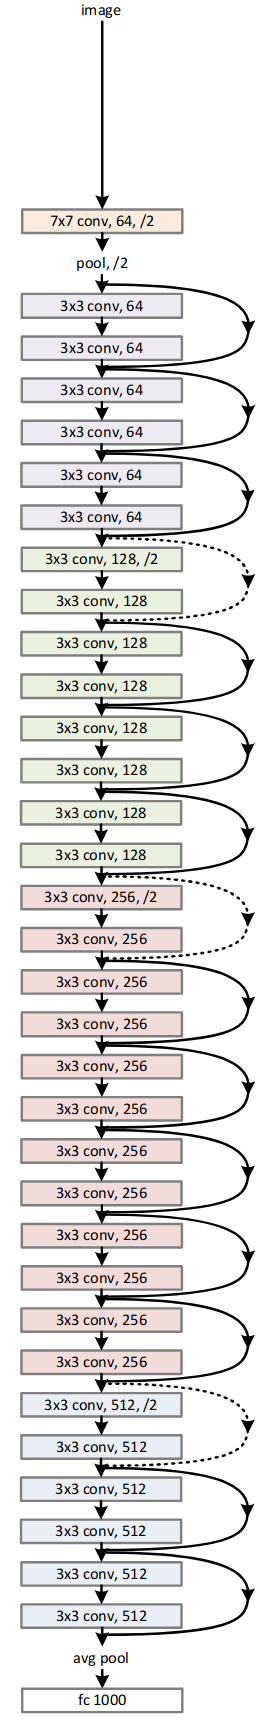
\includegraphics[width=0.2\textwidth]{images/Screenshot-20230207144959-265x1725.png}
    }
    \caption{Diagram for the ResNet34 model. Curved arrows represent a residual connection, with dotted arrows meaning the connection also downsamples the input. The four encoder blocks are colored differently. For use as an encoder, the fully connected layer at the end is omitted. Image taken from \cite{heDeepResidualLearning2015}}
    \label{fig:resnet34}
\end{figure}

    \chapter{Techniques used to improve model accuracy}
    \label{sec:techniques}
    Basic steps such as optimizing parameters for training are not the only methods available to try to improve the performance of the resulting model. 
Other techniques may be used to achieve better results, either by facilitating learning in some way or exploiting more data. 
In the following sections, the techniques employed during model development in this thesis will be explained more in depth.
    \section{Transfer Learning}
\label{sec:transfer_learning}

Coming back to the human learning analogy, it is often the case that knowledge or skills gained in one field can be applied to other fields, without having a lot of experience in these new disciplines. For example one might take their knowledge about composition from drawing to apply it to taking good pictures in photography. Although the technical details of both fields are different, they have some shared concepts, which help a person proficient in one to perform well in the other. That same person might also be able to improve in this new discipline faster than others, who do not have any applicable prior knowledge, because they can focus on learning other key skills needed to excel.

\emph{Transfer leaning} is the idea to apply this concept to neural network training. From a high level perspective, what happens during computation in a neural network, is that each layer transforms the input into an \emph{intermediate representation} of the data, which extracts different features present in the input. For example, one layer might learn to detect edges, which the next layer then combines to knowledge about the location of corners. As you can imagine, these types of features are useful for recognizing objects, such as a tennis ball, in a picture. It also stands to reason that these same features would be useful to detect circular droplets. The extracted features are rarely this clear cut or human-understandable as in this example, but the point remains the same. 

Using a model trained on one dataset and using these weights as a starting point to fine tune the model on the actual problem dataset is also called \emph{pretraining}. This is especially useful if the data for the target problem is scarce, as pretraining is often done on very large datasets such as \emph{ImageNet}\cite{dengImageNetLargescaleHierarchical2009}, which features over 14 million images (smaller subsets available) annotated for \emph{image classification}.
If the target problem is similar to the problem the model was pretrained on, the whole model can be used as a starting point for training. 
However, pretraining is also possible on a task different from the actual problem, in which case the pretrained model can only be used in a larger ensemble.

Pretrained weights for popular architectures are readily available for download and are employed in this thesis by using them as a feature extractor in an \emph{encoder-decoder} architecture (see section \ref{sec:architectures})

There are other forms of transfer learning, such as \emph{knowledge distillation}, where the concept is to use a complex model that is well adapted to the task to train a comparatively smaller model. The larger model has a higher knowledge capacity, but not all of this capacity has learned important knowledge. When training the smaller model on the soft outputs (before argmax) of the larger model, it may learn correlations which it might not have been able to learn on its own given its limited capacity. The smaller network could then be deployed instead of the larger one to save computation resources on weaker hardware.

In this thesis pretraining is used in two places. Firstly, for the encoder module of the U-Net architecture, a ResNet that is pretrained on the ImageNet dataset is used. Secondly, the experiments examine if pretraining the model on the Cityscapes dataset helps to improve performance on the vapour image dataset.
    \subsection{The mean teacher approach to semi supervised learning}
\label{sec:mean_teacher}

As mentioned multiple times already, the starting hurdle for building machine learning solutions is obtaining enough high quality annotated data. 
For image segmentation tasks, this means segmentation masks, which are notoriously time consuming to produce. 
In our case, no annotated data was present in the beginning and it would be unreasonable to spend a large amount of time to annotate a lot of images, so only a limited amount of labeled samples were produced. 
In contrast, unlabeled images can be obtained very quickly and in large amounts, as one good measurement run can produce hundreds to thousands of images (even though not all of them may be usable).

Thus it would be very beneficial if we could make use of this unlabeled data in some way during training. 
Approaches to learning that utilize both labeled and unlabeled data are called \emph{semi-supervised learning}, in contrast to \emph{(fully-)supervised} or \emph{unsupervised learning}, where only labeled or no labeled data is used respectively. 
One example for such a procedure is called the \emph{Mean Teacher approach}.\cite{tarvainenMeanTeachersAre2018}

The main idea of the Mean Teacher approach it to use two models, one \emph{student} and one \emph{teacher}, and have the student learn from examples produced by the teacher.

The reason unlabeled data is not directly usable for model training is that no classification cost can be applied to the outputs, as the target is undefined.
While there is no way to automatically generate a 100\% accurate target, as this is essentially what we try to train our model to do, when we look at it the other way around, we can use a model to approximate the target to a degree.
However, using the same model we want to train to simply approximate its own training samples would not provide any benefit.
Two steps are are used in the Mean Teacher method to still make use of these kinds of \emph{pseudolabels}.

As mentioned in \ref{sec:training}, augmentation and regularization techniques have the purpose of enabling the model to learn the concept of its target function more broadly, since small variances in the input should still produce a similar output. 
This can be applied not only when comparing the output of the model to the ground truth, but also when comparing the outputs of the model for the same input data, but different levels of noise. 
In a sense, if the model has properly learned the correct abstractions, its prediction should be similar, even if the input is slightly different.
What this means concreetly in this case, is that the method uses the teacher to make a prediction on an input without any noise and then computes student predicitons on the same input to which  augmentations have been applied.
In general, the teacher should have an easier time to predict accurate labels for a sample without noise, so a slightly better approximation of the theoretical correct labels should be produced. 
A \emph{consistency cost} can then be applied between student and teacher predictions which are then used in the same way as the \emph{classification cost} to update student weights.

Another way to improve the relative quality of the pseudolabels is to improve the teacher model they are generated by.
This is where the second key concept of the method comes in.
Instead of using the same weigths for both student and teacher models, the \emph{exponential moving average} (EMA) of the student weights are used for the teacher.
What this means is, if $\theta_t$ are the weights of the student at step $t$ and $\theta'_t$ are teacher weights at the same point, $\theta'_{t+1}$ is defined as follows:
$$
    \theta'_{t + 1} = \alpha\theta'_t + (1 - \alpha) \theta_t
$$
where $\alpha$ is a smoothing coefficient called the \emph{EMA decay}.

The EMA of a model has been observed to be slightly better than the model itself, as well as being more stable during the training process, since changes to the student model are only adapted slowly. Combining this with the noisy student inputs makes it possible to extract a lot of improvment from unlabeled examples, but can also be applied during training steps with labeled data. 

\begin{figure}[htbp]
   \makebox[\textwidth][c]{
        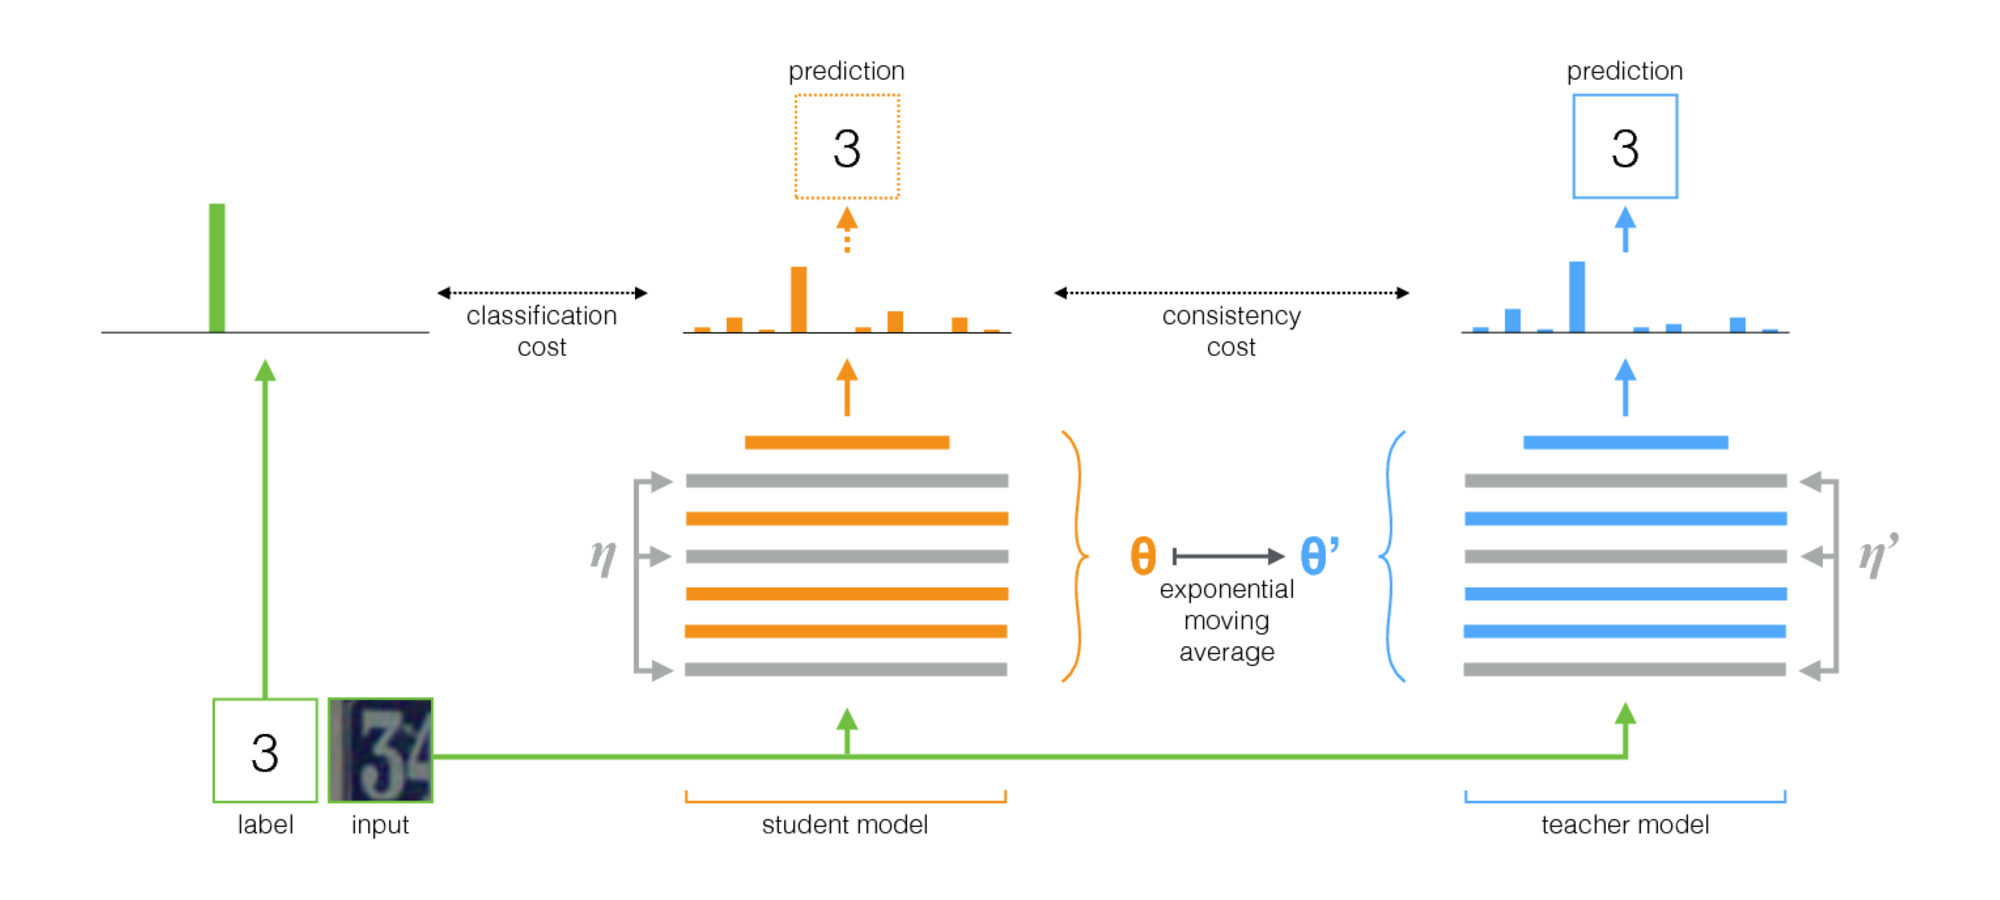
\includegraphics[width=\textwidth]{images/mean_teacher.png}
   }
   \caption{Schematic depiction of the Mean Teacher method. The graphic illustrates a single training step with one labeled sample for the image classification task. The classification loss is applied between the ground truth and the model predictions, while the consistency cost is computed between the soft outputs of both models. After updating the student weights, new teacher weights are computed as the EMA of the student weights. Steps with unlabeled samples simply omit the classification cost. Image taken from \cite{tarvainenMeanTeachersAre2018}}
   \label{fig:mean_teacher}
\end{figure}

During traing, it is necessary to apply a relative weight between classification loss and consistency loss, since initially, the teacher model may produce very bad outputs and which might also differ a lot from the student outputs, since no concepts haven been learned yet. 
If the consistency is given too much weight the model will prioritize being consistent with the teacher over predicting the correct classes for the labeled examples, potentially hurting or preventing any training progress. 
Thus, the weight of the consistency loss should start low and be slowly ramped up over the period of the training. 

Another key aspect of the method is considering which augmentations are chosen for the student inputs. To produce a large enough difference between outputs, strong augmentations are necessary to achieve the best improvements. The augmentations should also be well tailored to the dataset that is being trained on. 

Lastly, as mentioned above, the method introduces the hyperparameter $\alpha$ into the training, which has a big influence over the improvement that can be achieved. If it is too low, the benefits of using the EMA may not be present as much, since the teacher is too similar to the student. If it is too high, the teacher may not be updated quickly enough to incorporate the students improvement. 

The applicability of the mean teacher method will be more closely examined during the experiments of the thesis, with the goal to improve overall accuracy as well as generalization of the model produced. 

    \chapter{Droplet detection}
    \label{sec:detection}
    Before discussing the experiments conducted in this work, it is important to understand in which context the final model will be used to process experimental data. The following section also discusses the limitations of the model and the experimental setup.

\section{Detection and measurement algorithm}
\label{sec:algorithm}

The measurement process consists of several steps, each employing different techniques to improve measurement accuracy and reduce computation time.

\paragraph{Step 1: Image preprocessing} is done on the raw image data. This step is done to improve visibility of the droplets in the image and make a first guess as to which images actually contain droplets. 
The preprocessing is done batched by calculating the mean image $\mathbf{m}\in\mathbb{R}^{H\times W}$ as well as the mean greyscale value $\mu\in\mathbb{R}$ of the batch $\mathbf{B}\in\mathbb{R}^{N\times H\times W}$, subtracting $\mathbf{m}$ from each image in the batch, adding $\mu$ to each pixel and then mapping the resulting values to the interval $[0,255]$.
This process must be done batched because of memory constraints, but batching the images also has the advantage that images in one batch are more likely to be similar to each other in terms of lighting conditions, which makes the output more consistent.
This only applies if the images are taken in one measurement run, which is the intended use case.

The mean image subtraction is done to remove camera and lens artifacts such as hot pixels or dust from the images.
This is not primarily done to improve the models detection accuracy, but in order to filter out images that are not suitable for further processing.
The metric for deciding if an image contains any structure that could be a droplet is the \emph{Michelson contrast}, which is defined as 
$$
    C = \frac{I_\text{max}-I_\text{min}}{I_\text{max}+I_\text{min}},
$$
where $I_\text{max}$ and $I_\text{min}$ are the maximum and minimum luminance values in the image.
Since droplets have very dark and very bright regions, they produce a high Michelson contrast.
Images aren't considered for further processing if $C$ is below a certain threshold.
The reason artifacts need to be removed is that the they are very dark compared to the background, which means even images without any droplet structures will have a high Michelson contrast.

Lastly, before applying the model to the images, they are normalized to have a mean of 0 and a standard deviation of 1 using ImageNet mean and standard deviation to match the training augmentations.

Training data underwent the same preprocessing steps.

\paragraph{Step 2: Droplet detection} is done by a model trained to identify droplets with dark borders and bright centers as in-focus and segment the images into three classes, \emph{droplet border}, \emph{droplet inside} and \emph{background}.
Segmenting the images into three classes instead of two is important in the next step, since it helps to detect errors the model makes in the segmentation process.

Details on model training and evaluation can be found in section \ref{sec:experiments}.

\paragraph{Step 3: Droplet measurement} is done by first grouping all adjacent pixels labeled as \emph{droplet border} in the segmented image to distinct instances. 
This is essentially done by choosing a starting pixel with the correct label and scanning its neighboring pixels to find all pixels that are also labeled as \emph{droplet border}.
This step is repeated for this new set of pixels until no more pixels with the correct label can be found.
The process starts again for a new pixel that has not been assigned to a droplet yet, until all labeled pixels have been processed.
The library \emph{scikit-image}\cite{waltScikitimageImageProcessing2014} used to accomplish this employs several tricks to speed up this process \cite{wuOptimizingConnectedComponent2005}. 

As a first filtering step, all areas that are smaller than a certain threshold are now discarded, since no droplets below a certain size can be expected to fit the criteria for being in focus.
For each remaining area, the locations of all pixels are averaged to locate the center of the droplet.
Since the droplet is approximately circular, the average distance of all pixels from the center is calculated and used as a measure for the radius of the droplet.
Because the border of the droplet has a certain width and labels sometimes extend beyond the actual droplet, only the values between the 80th and 95th percentile of the distances are used to calculate the radius.

\section{Common problems and limitations}
\label{sec:limitations}

The model used to segment the image is not perfect, which means that sometimes areas which do not belong to a droplet are labeled as \emph{droplet border} or \emph{droplet inside} or the model fails to detect a droplet that is actually present in the image.
In this section, the most common errors are discussed and possible solutions are proposed, some of which are implemented already.

\paragraph{The model labels an out of focus droplet or other noise partially with border and center labels.}
\label{sec:partially_wrong}
This is the most common error observed when applying the model to experimental data, examples for which can be seen in Figure~\ref{fig:partially_wrong}.
The model will assign a border label to the dark pixels of an out of focus droplet or a center label to brighter areas of the image that are not part of a droplet, possibly even both for the same structure.
However, this will very rarely happen in a way in which the border region completely surrounds the center region in a closed shape, which can be used to filter out these errors.

\begin{figure}[htbp]
    \centering
    \begin{tabular}{ll}
        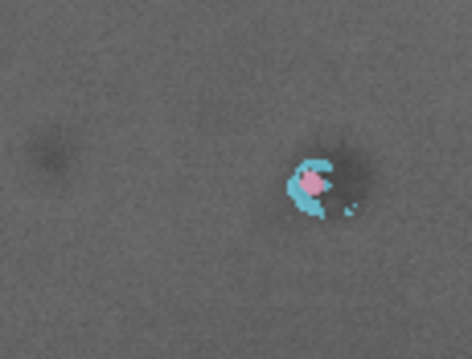
\includegraphics[width=0.4\textwidth]{images/bad1.png}
        &
        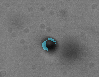
\includegraphics[width=0.35\textwidth]{images/bad2.png}
    \end{tabular}
    \caption{Example images showing a labeling error as described in section \ref{sec:partially_wrong}. Blue pixels represent \emph{droplet border} labels, and pink pixels represent \emph{droplet inside} labels.}
    \label{fig:partially_wrong}
\end{figure}

Training the model to assign two different labels for the droplets instead of one allows the criterion of droplets having a closed border around a center region to be used not only during training, but also after segmentation.
To check if a border area such as the ones described in Figure~\ref{sec:algorithm} fulfills this criterion, the algorithm calculates its \emph{alpha shape}\cite{edelsbrunnerShapeSetPoints1983a} and then checks if any of the pixels inside the shape are labeled as \emph{droplet inside}.

The alpha shape of a set of points is a generalization of their \emph{convex hull} and for a real number $\alpha$ includes all edges between the points for which a \emph{generalized disk} with radius $\frac{1}{\alpha}$ can be drawn so that the points of the edge lie on its border and the disk contains no other points. For $\alpha=0$, the generalized disk becomes a half-plane and the alpha shape is equivalent to the convex hull. In the code, the alpha shape is calculated using the \emph{alphashape}\cite{bellockBellockkAlphashapeV12021} package, which first calculates the \emph{Delaunay triangulation} of the points and then uses the criterion described above to determine which edges to include in the shape. The parameter $\alpha = 1$ is used since the pixel coordinates are discrete and the pixels are directly adjacent to each other. 

This method of filtering works very well for any but the most extreme cases and improves the accuracy of the measuring process significantly.

\paragraph{The model labels an out of focus droplet or other noise completely with border and center labels.}

This is a much rarer error than the one described in the previous paragraph, but it can still happen. 
It is mostly encountered when the image is very dark overall, which ironically causes the preprocessing step described in section \ref{sec:algorithm} to produce bright artifacts in such images, instead of removing dark spots. 
One example of such an image can be seen in Figure~\ref{fig:totally_wrong_a}.
Since the model identifies in-focus droplets by their bright center, this behaviour is not completely unexpected.

However, very rarely the model will assign a false positive even to an area which is not significantly brighter than the background, as can be seen in Figure~\ref{fig:totally_wrong_b}.

\begin{figure}[htbp]
    \centering
    \begin{subfigure}{\textwidth}
        \makebox[\textwidth][c]{
            \begin{tabular}{ll}
                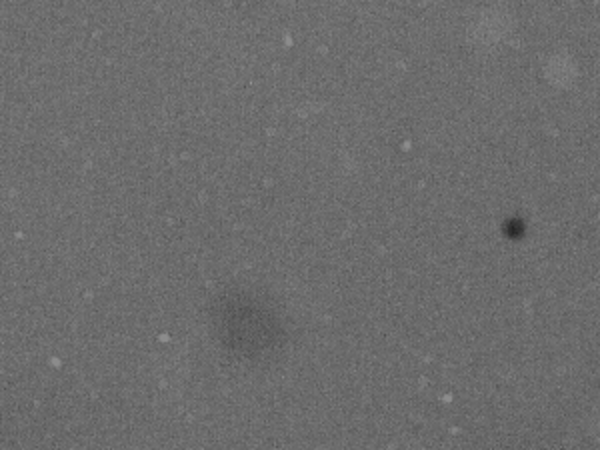
\includegraphics[width=0.45\textwidth]{images/bad4_pic.png}
                &
                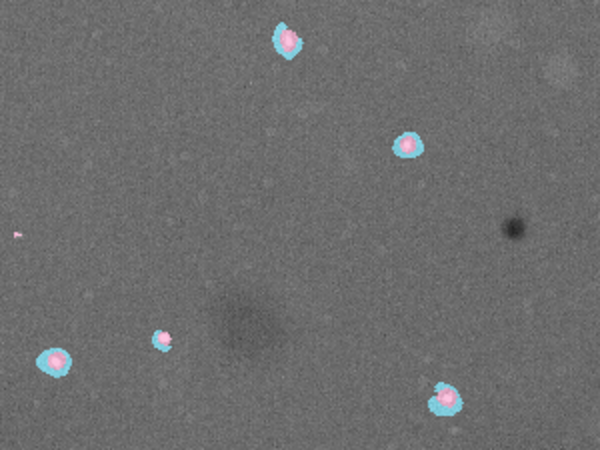
\includegraphics[width=0.45\textwidth]{images/bad4_mask.png}
            \end{tabular}
        }
        \caption{The model identifying bright artifacts in dark images as droplets. Note that only bottom left and top right labels are fully closed shapes, which can't be filtered out.}
        \label{fig:totally_wrong_a}
    \end{subfigure}
    \begin{subfigure}{\textwidth}
        \makebox[\textwidth][c]{
            \begin{tabular}{ll}
                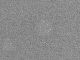
\includegraphics[width=0.45\textwidth]{images/bad3_pic.png}
                &
                
\includegraphics[width=0.45\textwidth]{images/bad3_mask.png}
            \end{tabular}
        }
        \caption{The model identifying a comparatively brighter spot as a droplet.}
        \label{fig:totally_wrong_b}
    \end{subfigure}
    \vspace{0.2cm}
    \caption{Examples for cases where the model confidently labels an out of focus droplet or other noise completely with border and center labels. The left image shows the original image, the right image shows the segmentation mask. Blue pixels represent \emph{droplet border} labels, and pink pixels represent \emph{droplet inside} labels.}
    \label{fig:totally_wrong}
\end{figure}

This kind of error is much more severe, since there aren't any criteria to differentiate these kinds of false positives from the structure of the actual droplet labels.
Thus, the only way to mitigate this that comes to mind are improving image preprocessing and/or training the model differently to not make these kinds of mistakes.

One idea to improve the preprocessing is to use a different technique for removing the artifacts. 
The current method of removing the artifacts by subtracting the background image from the original image is very simple and works well if the images in the batch are similar in brightness, but it is not very robust to outliers.
A different approach then, would be to use the background image as a mask for identifying artifact locations instead, and overwrite the pixels in the original image with a more appropriate value. 
This could either be the mean brightness of each individual image, or the values at the same pixel location in the original image with a gaussian blur applied to it.
A process like this could help in minimizing bright artifacts, which seem to be the main cause of this kind of error.
For this, \emph{inpainting methods} \cite{OpenCVImageInpainting,teleaImageInpaintingTechnique2004,bertalmioNavierstokesFluidDynamics2001} could do a good job, however they were found to be too computationally expensive for the task at hand.

To instead make the model more robust to these kinds of artifacts, some kind of data augmentation could be used that mimics the effect of the artifacts, such as \emph{salt-and-pepper/binary noise}. Another option would be to explicitly use additional samples of images the model seems to find difficult to classify correctly, such as the ones shown in Figure~\ref{fig:totally_wrong}. These examples would need to be labeled of course, but could potentially improve the model substantially in this regard.

\paragraph{Very fast droplets} that travel a significant distance in the time it takes to expose the image (inv. proportional to \emph{shutter speed}) appear as streaks instead of circles. 
Since the model is trained to identify droplets that are ellipsoidal in shape, it won't be able to label those streaks correctly.
The structure of these streaks is also much less distinct than the structure of the droplets, which makes it harder to say if a streak is in focus or not.

Up to a point, this can be mitigated by increasing the shutter speed during image capturing, however this will also decrease the amount of light that reaches the camera, making the images darker overall, so depending on the lighting conditions, this may not be a viable option.

Using a different model that is trained to identify streaks instead of circles or even training the same model to segment streaks into a different class could be a solution to this problem. 

Doing this could have some additional benefits.
For example, by finding the minimum angled rectangle that contains the streak we could calculate the ratio of the width and height of the rectangle to estimate the speed of the droplet, since the shutter speed is a known parameter and the longer side of the rectangle corresponds to the distance the droplet traveled in the time it took to expose the image.
Since the speed of the droplet is another interesting parameter to measure, this could be a useful addition to the model.
One might even be able to deliberately lower the shutter speed to make the droplets appear as streaks for the purpose of measuring the distribution of the droplet velocity.

Due to time constraints, this idea couldn't be explored further in this thesis, but could be an interesting topic for future work.

\paragraph{Droplets that are too small} are not reliably identified by the model, since the smaller the droplet, the less distinguishable the different parts of the droplet become. 
This is an inherent problem of techniques using imaging as a measurement method, since there is always a limit to the scale at which objects can be resolved.

Up to a point this can still be mitigated by increasing the resolution of the camera or the magnification of the lens, but this will also increase the cost of the setup and will only be possible to a certain extent.

Since this problem isn't something that is specific to the algorithm, but rather a limitation of the imaging technique itself, there isn't much that can be done to improve the model in this regard.
For the actual usage of the technique, this means human oversight is still necessary for deciding if the approach is applicable to specific set of captured data.

\paragraph{In focus criteria may be unrepresentative of actual in focus droplets.} Instead of an error observed in the measuring process, this is a potential problem with the method itself.
Which droplets are considered in focus and should be included in the measurement is a key aspect of the process, since data has to be labeled accordingly. Structures with extremely sharp corners are exceedingly rare in the data captured by the experimental setup, which is why \Citeauthor{kapplAkustischInduzierteVernebelung2022}\cite{kapplAkustischInduzierteVernebelung2022} argues that structures with a dark border and a bright center should be considered sufficiently in focus.

The reasoning behind this is that light that passes through the outer areas of the droplet is scattered more strongly, resulting in less light reaching the camera, while light that passes through the center of the droplet passes through straight, with beams near the center even being focused slightly.

The success of the method as a measurement technique depends heavily on the veracity of this assumption. 
However, if in the future, other criterions are found to be more suitable to differentiate between in focus and out of focus droplets, the method could theoretically be adapted to use those instead.
    \section{Experimental Setup}
\label{sec:setup}

Athough the detection techniques described in \ref{sec:detection} are in principle adaptable to similar data, the image data used in this thesis is captured using a specific setup. 

The setup uses the \emph{Fastcam Mini UX} in combination with a \emph{Olympus LMPlan IR 50X / 0.55} microscope objective lens as well as a seperate focussing lens to capture images of the droplets.
Together with a parallel light source, this setup forms a microscope with a large magnification factor, which is necessary to capture the droplets in sufficient detail considering their expected size of \SIrange{1}{30}{\micro\meter} \cite{kapplAkustischInduzierteVernebelung2022}.

The SAW device together with a liquid reservoir is placed next to the light source and the camera so that the droplet droplet stream is illuminated from the side. An image of the setup is shown in \ref{fig:setup}.

Images are taken at a resolution of \qtyproduct{1280 x 1024}{\pixel} and a frame rate of \SI{50}{\hertz}. The framerate is kept low to enable capturing data over a longer period of time without saturating the memory of the camera, since the droplets are not constantly in the field of view of the microscope. 

\begin{figure}[htbp]
    \centering
    \makebox[\textwidth][c]{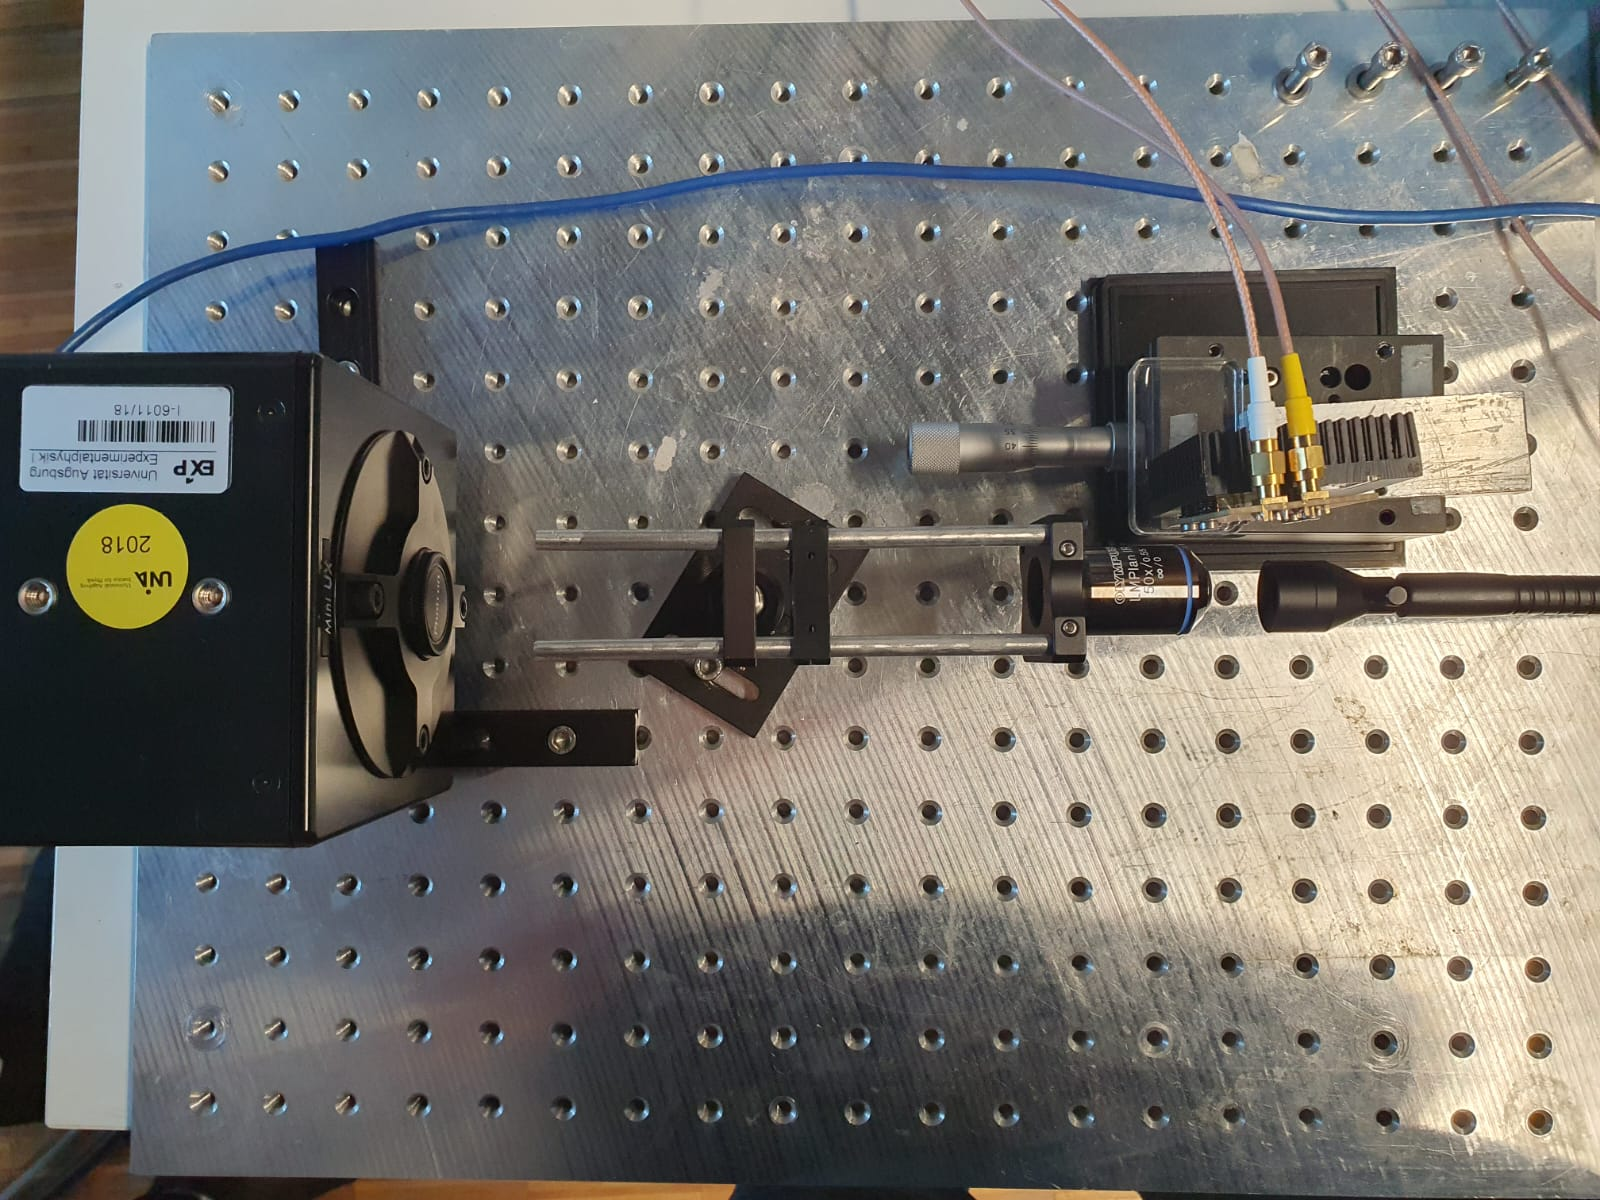
\includegraphics[width=0.9\textwidth]{images/0c35c5ed-b77b-4d8d-b30f-b23403bd04d0.JPG}}
    \vspace{0.2cm}
    \caption{Image of the measurement setup. From left to right the high speed camera, the focusing lens and objective lens, the SAW device and the liquid reservoir as well as the light source are visible.}
    \label{fig:setup}
\end{figure}

    \chapter{Experiments and Results}
    \label{sec:experiments}
    Several techniques are explored during model training in the hopes of improving the detection and measurement performance as well as how the model generalizes. 
This section evaluates the results of these experiments and discusses their effectiveness.

Before discussing specific experiments, the general training and evaluation environment will described.

\paragraph*{Training and Evaluation Setup}
All learning is done using the \emph{pytorch}\cite{paszkePyTorchImperativeStyle2019a} framework.

Where applicable, techniques were tested on the \emph{Cityscapes}\cite{cordtsCityscapesDatasetSemantic2016a} dataset, which contains 3000 images with pixel-level annotations of 30 different classes, 19 of which were used during training and evaluation.
Since the annotations for the Cityscapes test set are not public, models trained on this dataset are only evaluated based on their performance on the validation data. 

The training data for the target dataset contains image data recorded using the setup described in \ref{sec:setup} with three different sets of imaging and droplet generation parameters. The data is annotated with three classes, namely \emph{droplet inside}, \emph{droplet outside} and \emph{background}. Annotation was performed with the Software \emph{CVAT}\cite{CVAT_ai_Corporation_Computer_Vision_Annotation_2022}.

The test set for the vapour data contains 35 images from different experiments, which were not used during training. The images in the test set are carefully selected to cover a wide range of droplet sizes and clarity as well as different overall lighting conditions. It also deliberately includes images with a lot of artifacts and noise that are observed to commonly cause problems for the model (see \ref{sec:limitations}) as well as images with no droplets at all.

The loss function used for training is the \emph{cross entropy loss} which is defined as:
\begin{equation*}
    \ell_{i, j} = -\log\hat{y}_{i, j, y_{i, j}}\quad,
\end{equation*}
where $\hat{y} \in \mathbb{R}^{M \times N \times C}$ are the predicted class probabilities, $y \in \mathbb{N}^{N \times M}$ is the ground truth class label and $C$ is the number of classes. The loss is averaged over all pixels \cite{CrossEntropyLossPyTorch13}.
\begin{equation*}
    \mathcal{L}(y, \hat{y}) = \frac{1}{MN} \sum_{i=1}^M \sum_{j=1}^N \ell_{i, j}
\end{equation*}
The class probabilities are calculated from the logit outputs $o$ of the model using the \emph{softmax} function:
\begin{equation*}
    \hat{y}_{i, j, c} = \frac{\exp(o_{i, j, c})}{\sum_{k=1}^C \exp(o_{i, j, k})}\quad.
\end{equation*}

The main metric used for evaluating the performance of the model is the \emph{mean intersection over union} (mIoU, see \ref{sec:imseg}), which is calculated by accumulating the intersection and union for each class over the whole data set, calculating the class-wise IoU and then averaging the results over the number of classes.  

For training on the vapour dataset, additional metrics can be calculated which may better reflect the models performance in its intended application. To do that, the measurement algorithm is applied to both the predicted and ground truth segmentation masks. Predicted droplets are considered to be correctly detected if their center is within a the area of a ground truth droplet, which is precise enough because the droplets are generally very sparsely distributed.
The additional metrics calculated from this information are 
\begin{itemize}
    \item \emph{Precision}: The fraction of detected droplets (P) that are actually present in the image (TP). $$\frac{\text{TP}}{\text{P}}$$
    \item \emph{Recall}: The fraction of actual droplets (= T) that are detected. $$\frac{\text{TP}}{\text{T}}$$
    \item \emph{Relative Mean Radius Error} (RMRE): The relative difference between the predicted and ground truth average droplet radius (ADR). $$\frac{\text{ADR}_\text{pred}}{\text{ADR}_\text{truth}}$$
    This is calculated considering only the droplets that are detected in both the ground truth and the prediction (RMRE$_\text{c}$) as well as all droplets that are present in the ground truth (RMRE$_\text{t}$).
\end{itemize}
Unless stated otherwise, all metrics are calculated for the test set of the vapour dataset.

All training uses \emph{early stopping} to determine the end of training. The model is trained for as long as the improvement in the evaluation metric (mIoU) is significant. Improvement is considered stagnant if the metric doesn't surpass its best value by at least a certain \emph{minimum delta} within a certain number of \emph{patience} epochs. Patience and minimum delta are generally set to 30 and \num{1e-4} respectively.

Additionally, the model is trained using a \emph{learning rate scheduler} which reduces the learning rate by a certain factor if the improvement in the evaluation metric is not significant for a certain number of epochs. The idea behind this is that initially a higher learning rate is beneficial to avoid getting stuck in local minima. However, in later stages of training the model may aleady be close to a global minimum and a higher learning rate may cause it to overshoot the minimum, so lowering the learning rate helps to avoid this. The scheduling process used in this thesis is called \emph{ReduceLROnPlateau}. There are more sophisticated approaches to scheduling, however the ReduceLROnPlateau scheduler achieves good results in this case and is easy to implement without knowing the exact number of epochs that will be needed for training.

Unless otherwise stated the model architecture is always a U-Net with a ResNet34D pretrained on ImageNet data as its encoder.
    \section{Oversampling to overcome class imbalance}
\label{sec:oversampling}

Class imbalance is a common problem in many machine learning tasks.
This is especially true in the case of the underrepresented classes being the most relevant ones, as is the case for the droplets in the vapour dataset.
The background label makes up \SI{99.914}{\percent} of all labeled pixels in the dataset, while the droplet border and droplet inside labels only make up \SI{0.063}{\percent} and \SI{0.023}{\percent} respectively.

Initially, this extreme unbalance made it impossible to train a model that could detect droplets and the mIoU would stagnate around \num{0.33}, which is the accuracy of a model that always predicts the background class.

One way to combat this imbalance is weighting the loss function of each class inversely proportional to the number of samples in the dataset that belong to that class, to prioritize predicting the underrepresented classes correctly during training. 
However, perhaps due to the unusually large imbalance, this method did not improve the performance of the model. Using smaller weights than the inverse distributions didn't achieve better results either.

The method that is applied in the thesis to overcome this problem is a form of \emph{oversampling}\cite{mohammedMachineLearningOversampling2020}, where the occurence of the underrepresented classes is artificially increased by showing the model samples that do contain these classes more often.
Although there are more sophisticated approaches to oversampling \cite{ReviewImbalancedData2017}, the solution used in this thesis is a simple one that is easy to implement, but has proven to be effective.

Since droplets are distributed very sparsely in the data, when splitting the images into smaller samples, a lot of the splits will not contain any droplets. 
Instead of including these empty regions in the training set, they are discarded when the split images are created.
Doing this changes the label distribution to \SI{99.84}{\percent} background, \SI{
0.116}{\percent} droplet border and \SI{0.044}{\percent} droplet inside, which doesn't appear to be much better than the original distribution, but roughly doubles the occurence rate of the droplet classes. 
This alone is enough to allow the model to learn to detect droplets with good accuracy.

To take this further, instead of splitting the image dimensions by two they could also be split by a larger factor, which would increase the relative density of droplets in the samples even more.
The results of this are shown in each experiment seperately, since the same split factor might not work well for all approaches.
No split factors larger than 4 were tested, since images would become very small and split droplets into different samples more often, which might also be detrimental. 

No further comparative studies were conducted to determine the optimal split factor or the best way to apply oversampling, since the results of this simple approach were already good enough to be used in the thesis.
Oversampling is used in all other experiments, since training on the vapour dataset is impossible without it.


    \section{Mean Teacher for general improvement}
\label{sec:mean_teacher_general}

As described in \ref{sec:mean_teacher}, the mean teacher approach should enable us to utilize unlabeled data to improve the performance of our model.
To verify the effectiveness of this approach, the method is first tested on the Cityscapes dataset before it is applied to the vapour dataset.

In this experiment, the only concern is to improve the general performance of the model measured by the metrics described above. 
Further experiments will verify the effectiveness of the method for improving the generalization capabilities of the model on the vapour dataset.

\paragraph{Verification on Cityscapes} 

For the Cityscapes dataset training is done on images downsampled to a \qtyproduct{256 x 512}{\pixel} resolution. The initial learning rate is set to \num{1e-3} and the batch size to 16 containing 4 labeled and 12 unlabeled samples. The patience for the scheduler is set to 5 epochs and the reduction factor is set to \num{0.1}.
The weight of the consistency loss is ramped up to its maximum value of \num{1.0} over the first 15 epochs using a sigmoid ramp.
Consistency loss is calculated using the \emph{cross entropy loss} between the predictions of the student and the hard predictions of the teacher (meaning after applying \emph{argmax}).
The teacher is updated using an EMA with a decay $\alpha$ of \num{0.996}.

For the baseline model, the best results are achieved by using an initial learning rate of \num{1e-4} with a batch size of 16, a scheduler patience of 20 epochs and a reduction factor of \num{0.5}. 

The baseline model is trained on 100 labeled samples from the training set, while the mean teacher model is trained on the same 100 lableled samples plus all other samples from the training set as unlabeled samples.
A training epoch when using MT is considered to be finished when the model has seen all unlabeled samples once, with the labeled samples being seen as many times as necessary to fill the batch size. This means epochs for MT training contain considerably more samples than epochs for baseline training, which is why the patience value for baseline training is higher.

For the baseline model, the augmentation pipeline consists of a random \numproduct{224 x 224} crop, a random translation, scaling and rotation with a probability of \num{0.5}, a RGB-shift with a probability of \num{0.5} and a random variation of the image brightness and contrast with a probability of \num{0.5}.  

The augmentation pipeline for the MT training employs a different set of augmentations, since strong asymmetrical augmentations between teacher and student are important for the MT approach to properly function. For this, the augmentation pipeline is inspired by \Citeauthor{schererPseudoLabelNoiseSuppression2022}\cite{schererPseudoLabelNoiseSuppression2022}. It contains the same shift, scale, rotation and crop operations as the baseline augmentations, but also applies a strong dropout of \num{0.5} to the student model, as well as using a \emph{CowMask} technique to compose new samples by combining two images as well as their teacher predictions.
For this technique a mask such as the one shown in Figure \ref{fig:cowmask} is generated and applied to an image and its pseudo label. The same is done for a second image and its pseudo label with the inverted mask and both are combined.

Finally, the images are normalized using the mean and standard deviation of the ImageNet dataset in both baseline and MT training.

\begin{figure}[htbp]
    \centering
    \makebox[\textwidth][c]{
\includegraphics[width=0.4\textwidth]{images/Screenshot-20230221170853-829x417.png}}
    \vspace{0.1cm}
    \caption{Example for a cow mask used in the training process. The white areas mark regions that use the first image, while the black areas use the second image. From \cite{schererPseudoLabelNoiseSuppression2022}}
    \label{fig:cowmask}
\end{figure}

\paragraph{Results on Cityscapes}
With the MT approach, the model is able to achieve a mean IoU of \num{0.426} on the validation set, which is a significant improvement over the baseline model with a mean IoU of \num{0.349}.

However, this improvement is only achievable within a very small space of hyperparameters, as all training runs with different hyperparameters than described above yielded worse results than even the baseline model.

This deterioration in performance can likely be attributed to very poor pseudo label quality. As \citeauthor{schererPseudoLabelNoiseSuppression2022}\cite{schererPseudoLabelNoiseSuppression2022} discovered in their analysis of \emph{pseudo label filtering} techniques, pseudo labels with poor quality have a detrimental effect on final model performance.
Since the setup used in this thesis doesn't achieve very high performance on the Cityscapes dataset as is, even when using all labeled samples (mIoU of \num{0.475}), it stands to reason that label quality may hurt the training process if hyperparameters are suboptimal.

Nonetheless, the results of this experiment show that the MT approach is able to improve the performance of the model. With the supervised performance on the target dataset being signifcantly better than on the Cityscapes dataset, it is likely that the MT approach will be able to improve the performance of the model on the vapour dataset as well.

For a more comprehensive overview of training results, see Table \ref{tab:cityscapes_results_mt}.

\begin{table}[htbp]
    \centering
    \begin{tabular}{llllllllrr}
        \toprule
        \multicolumn{9}{l}{Cityscpapes Training}\\  
        \midrule
        Approach & \#lbls & lr & bsize & lrsf & lrsp & Dropout & $\alpha$ & Loss &
        mIoU \\
        \midrule 
        Baseline & all & $0.0001$ & $16$ & $0.5$ & $10$ & - & - & $0.216$ & $0.475$ \\
        MT & 100 & $0.001$ & $16$ & $0.1$ & $5$ & \num{0.5} & \num{0.996} & $0.644$ & $\mathbf{0.426}$ \\
        MT & 100 & $0.001$ & $16$ & $0.1$ & $5$ & \num{0.4} & \num{0.996} & $0.559$ & $0.412$ \\
        Baseline & 100 & $0.0001$ & $16$ & $0.5$ & $30$ & \num{0.2} & - & $0.444$ & $0.349$ \\
        Baseline & 100 & $0.0001$ & $16$ & $0.5$ & $30$ & - & - & $0.469$ & $0.331$ \\
        \bottomrule
    \end{tabular}
    \vspace{0.1cm}
    \caption{The best training results of the Mean Teacher approach on the Cityscapes dataset, as well as the supervised baseline performance along with important hyperparameters. For abbreviations refer to Table \ref{tab:abbreviations}.}
    \label{tab:cityscapes_results_mt}
\end{table}

\paragraph{Setup on vapour dataset}
The training setup for the vapour dataset is very similar to the Cityscapes setup, with the images being split in half along the vartical and horizontal axis and these 4 segments being used as seperate samples. The decision to split the images instead of resizing them was made because the relevant objects in the images are already quite small, so resizing them might make it impossible to detect some of them. This leaves us with \qtyproduct{640 x 512}{\pixel} images, which necessitated lowering the batch size to 12 for baseline training and 8 (2 labeled, 6 unlabeled) for MT training.
Learning rate was generally found to be optimal around \num{1e-3}.

Another difference in the setup is the augmentation pipeline, which is similar to the Cityscapes pipeline, but replaces the RGB-shift with gaussian noise, since the vapour dataset contains greyscale images. The gaussian noise might also be able to mimic some of the noise the camera produces, so it seems like an adequate replacement.
Furthermore, we also explore using \emph{CutMix}\cite{yunCutMixRegularizationStrategy2019} for mixing pseudo labels instead of the CowMask technique used for Cityscapes. 
CutMix cuts a rectangular region of the image instead of the varying sizes of blobs in the CowMask technique.
The reason this may be more suitable to the vapour dataset is that the objects in the images are generally quite small, so the CowMask technique, which masks generally smaller regions might not be effective in combining relevant features from the two images. On Cityscapes, CutMix was not attempted since \Citeauthor{schererPseudoLabelNoiseSuppression2022}\cite{schererPseudoLabelNoiseSuppression2022} already concluded that the CowMask technique was superior.

\paragraph{Results on vapour dataset}


    \section{Influence of pretraining on the model performance}
\label{sec:pretraining}

As mentioned in \ref{sec:transfer_learning} besides using a pretrained encoder, the thesis also explores pretraining the whole model on the Cityscapes dataset as a starting point for training on the droplet dataset.

Because the model has already learned some useful features, this could potentially speed up the training process and improve the performance of the model. 

This, the weights of best performing model on Cityscapes (mIoU \num{0.475}) is loaded when starting training, except for the last layer, whose number of output channels is changed to match the number of classes in the droplet dataset.

\paragraph{Results}


    \section{Mean Teacher for generalization}
\label{sec:generalization}

Another hope for the MT approach is that it will be able to improve the generalization capabilities of the model. Since different imaging parameters or different SAW devices will produce slightly different images, being able to adapt the model to new parameters without having to label new data would be a huge advantage.

To explore this, two subsets (S1 and S2) of the vapour datasets with different parameters are used to create two new datasets (DS1 and DS2). DS1 contains the labeled samples from S1 as well as samples from S2 with the labels removed. DS2 is built in the same way, but with S2 as the labeled dataset and S1 as the unlabeled dataset.

The model is then trained on one of the two datasets (DS1 or DS2) and evaluated on the validation set of the subset that was not included as labeled data (S2 or S1). Training is done once with only the labeled samples and once with the unlabeled samples using MT. This is repeated for both datasets, so that one model is trained on either dataset. 

To avoid adapting the model purely to one subset, the original test set is used for validation during training. 

A similar number of labeled ($\sim 30$) and unlabeled ($\sim 150$) samples are used for each dataset, so that the model is trained on the same number of samples in total.

If including the unlabeled samples from S2 helps the model improve on the test set of S2 compared to only having seen the labeled samples from S1 (and vice versa), it would indicate that the MT method does indeed help the model generalize without new labeled data.

Training parameters are the same as described in section \ref{sec:mean_teacher_general}.

\paragraph{Results}

The evaluation results are shown in table \ref{tab:generalization}. 
Unfortunately, the results aren't as conclusive as hoped. 
While using the unlabeled samples from S1 did help the model improve its mIoU on S1 (results for DS2 in Table~\ref{tab:generalization}), the opposite isn't true, with the supervised training on DS1 performing better than the MT training, although not as significantly. 
Additionally, in both cases the supervised model performs better in all measurement specific metrics except for the recall.

The reason for this could be that the data from S1 is generally more difficult to segment than the data from S2. 
This could mean that including the easier data from S2 as unlabeled data doesn't really help the model learn new information, while including S1 as unlabeled data (in the case of DS2) actually introduces new concepts to the model.
As evidence for the higher difficulty of S1, we can point to the mIoU on the Validation set during training being higher for DS1 than for DS2, where S1 samples were labeled.

To further investigate this in the future, we could construct another pair of datasets that achieve more similar scores on the original test set which could mean they are more similar in difficulty. 

As for now, evidence for the MT method's ability to help generalization without new labeled data is inconclusive. 

This doesn't discount the value of the MT method for improving the model in general, but could mean that including new data in the training means having to label a small fraction of it to enable the model to grasp its basic structure, which is still a huge advantage over having to annotate all of it.

\begin{table}[htbp]
    \centering
    \begin{tabular}{llllllll} 
        \toprule
        Set & MT  & Validation mIoU    & Test mIoU        & recall           & precision        & RMRE$_\text{c}$   & RMRE$_\text{t}$   \\ \midrule
        DS1 & no  & 0.76072          & \textbf{0.71120} & 0.70330          & \textbf{0.94118} & \textbf{-0.05730} & \textbf{-0.05524} \\
            & yes & \textbf{0.76570} & 0.70605          & \textbf{0.74725} & 0.89474          & -0.11600          & -0.14195          \\
        DS2 & no  & 0.72521          & 0.67748          & 0.62963          & \textbf{0.94444} & \textbf{-0.18807} & \textbf{-0.17170} \\
            & yes & \textbf{0.72534} & \textbf{0.71552} & \textbf{0.66667} & 0.85714          & -0.26960          & -0.25511          \\ \bottomrule
    \end{tabular}
    \vspace*{0.2cm}
    \caption{Training Results for the generalization experiments. The Set Column indicates which dataset was used for training and evaluation and refers to the sets described in section \ref{sec:generalization}. MT indicates whether the MT method was used. Bold values indicate the better result for each metric.}
    \label{tab:generalization}
\end{table}

    \section{Binary instead of multi-class segmentation}
\label{sec:binary}

In \ref{sec:algorithm} it's stated that training the model to segement the image into three different classes helps to filter out common model errors in later stages of the measurement algorithm. 
However, introducing a third class also makes the problem more difficult to learn. It could be that training the model on only two classes (background and in-focus droplet) would enable the model to avoid the errors in the first place, since it can learn the criterium for a droplet bein in focus more easily.

To test this, the model is trained on the vapour dataset, but with all different droplet labels combined into a single class. The model is then evaluated on the test set that underwent the same transformation. 

During the evaluation process, the filtering step performed by the droplet measurement algorithm is obviously skipped, since the inside labels don't exist anymore. 

Training parameters are the same as in \ref{sec:mean_teacher_general}.

\paragraph{Results}


    \section{Training with reduced layers}
\label{sec:reduced_layers}

The architecture of the model described in chapter \ref{sec:architectures} has five distinct downsampling and upsampling stages in its encoder and decoder paths respectively.
The stated purpose of the lower layers is to be able to utilize more contextual information since neurons in lower layers have a larger \emph{receptive field} than neurons in higher layers.

However, for our specific problem, objects are generally quite small  and the problem itself isn't very complex, so the contextual information provided by the lower layers might not be as useful as it is for larger objects.
Additionally, including the lower layers may not only be unnecessary, but also detrimental to the performance of the model, since it increases the number of parameters and with that the computational complexity, which makes it harder to train. 
This also plays a role in the demand for computational resources during training and inference, since even only omitting the deepest layers reduces the trainable parameter count from 24.5\,M to 9.1\,M.

To explore this hypothesis, the model is trained on the vapour dataset with the encoder and decoder paths reduced to only four/three stages each (final encoder stride is 16/8 instead of 32). The model is then evaluated as normal.

Because of time constraints, pretraining the reduced model on the Cityscapes dataset was not attempted, however since the Cityscapes dataset is much more complex than our own, it is unlikely the model would have achieved good results on it in the first place.

The experiment compares the performance with and without semi supervised learning, with a split factor of 2.

Training parameters are the same as described in section \ref{sec:mean_teacher_general}.

\paragraph{Results} of the experiment are shown in Table~\ref{tab:results_reduced_layers}. Comparison is done with the results of the complete model seen in Table~\ref{tab:vapour_results_mt}.

While the complete model still takes the top score when it comes to the mIoU metric (0.784 for supervised training with sf = 2, see Table~\ref{tab:vapour_results_mt}), the top result for the reduced model only lags behind slightly with 0.775 for the same training parameters (4 stages supervise sf=2, see Table~\ref{tab:results_reduced_layers}).

For the semi-supervised training, the reduced model consistently outperforms the complete model at the mIoU metric, with the only exception being the case where the 4-stage model is trained with sf = 4. 

What is most surprising is that this is true not only for the 4-stage model, but also for the 3-stage model, which only contains 1.7\,M trainable parameters.
While there is a slight drop in performance for 3 stages compared to 4, considering the difference in size between the two models, this is quite impressive.

Unfortunately, it seems the reduced models don't benefit from the MT approach for the RMRE metrics, as was observed in some cases for the complete model.

The best overall result is achieved by the 4-stage model during supervised training with sf = 2, which achieves a mIoU of 0.775 as well as precision and recall values of over 0.95, which is the highest combined accuracy observed.

Since the precision should reflect the actual performance of the model in the application very well, using this configuration for inference seems to be a good choice.

\begin{table}[htbp]
    \centering
    \begin{tabular}{lllllllll}
        \toprule
        \#Stgs./Param. & MT  & sf & Loss             & mIoU             & recall           & precision        & RMRE$_\text{c}$   & RMRE$_\text{t}$   \\ \midrule
        3 / 1.7\,M       & no  & 2  & 0.00103          & 0.75167          & 0.84667          & 0.97692          & -0.14081          & -0.13211          \\
                 &     & 4  & 0.00091          & 0.76490          & 0.86667          & 0.97744          & -0.12805          & -0.13039          \\
                 & yes & 2  & \textbf{0.00068} & 0.76703          & 0.85333          & \textbf{0.99225} & \textbf{-0.09556} & -0.10277          \\
                 &     & 4  & 0.00123          & 0.76038          & 0.91333          & 0.93197          & -0.10090          & -0.10861          \\ \midrule
        4 / 9.1\,M        & no  & 2  & 0.00077          & \textbf{0.77552} & 0.95333          & 0.97279          & -0.10466          & \textbf{-0.09549} \\
                 &     & 4  & 0.00088          & 0.76513          & 0.86000          & 0.94161          & -0.11796          & -0.10821          \\
                 & yes & 2  & 0.00084          & 0.76889          & 0.88000          & 0.97059          & -0.11428          & -0.11925          \\
                 &     & 4  & 0.00123          & 0.73325          & \textbf{0.96000} & 0.87805          & -0.10355          & -0.10079          \\ \bottomrule
        \end{tabular}
        \vspace{0.2cm}
    \caption{Evaluation results for models trained with a reduced number of encoder/decoder stages. CowMask is used as the mixing method. For comparison to full scale results refer to Table~\ref{tab:vapour_results_mt}. For abbreviations refer to Table \ref{tab:abbreviations}.}
    \label{tab:results_reduced_layers}
\end{table}


    \chapter{Conclusion}
    \label{sec:conclusion}
    This thesis explored the use of deep learning for the segmentation of droplets in images of fluids vaporized using surface acoustic waves.
The overall goal was to develop a model that can be used to detect the presence of droplets in such images and to employ it in a usable system that measures the size of the droplets.

It gave an overview to the physical background of the atomization techniques and mentioned some of the limitations of other measurement techniques.
Furthermore the basics of neural networks and deep learning as well as the concepts and structure of the employed architectures were explained.

An algorithm for the measurement of droplets from segmentation mask was developed and its shortcomings and strengths as well as possible improvements were discussed.

The thesis also explored the use of transfer learning and self-supervised learning to improve the performance of the model in its application.
While some of the techniques weren't as successful as expected, the results of the experiments still showed promise and possible future improvements were suggested.

As it stands, the thesis achieved its goal of building a tool that could find use in current research and development projects, while also providing a basis for further investigation and refinement.

The use of SAW for the application of atomization is a promising technique that has the potential to be used in a variety of applications and the author hopes that the work presented in this thesis will contribute to the development of this technology.

    \newpage 
%\nocite{*} 
\printbibliography[title={Bibliography}]

    \begin{appendices}
        \chapter{Abbreviations}
{
    \renewcommand*{\arraystretch}{1.1}
    \begin{table}[htbp]
        \centering
        \begin{tabular}{rp{0.6\textwidth}} 
            \toprule
            Abbreviation & Meaning\\
            \midrule 
            (D/F)CNN & (Deep-/Fully-) Convolutional Neural Network; a (deep) neural network that (only) includes convolutional layers in its main path\\
            SAW & Surface Acoustic Wave\\
            IDT & Interdigital Transducer\\
            lr & learning rate\\
            lrsp & learning rate scheduler patience\\
            lrsf & \linespread{1.0}\selectfont learning rate scheduler factor; the number the learning rate is multiplied by in case the scheduler detects stagnant progress\\
            bs, bsize & batch size\\
            lbls & labeled samples \\
            MT & Mean Teacher \\
            EMA & Exponential Moving Average \\
            sf & \linespread{1.0}\selectfont split factor; the number the height and width of the images and masks in the dataset are divided by for splitting them into smaller samples\\
            \bottomrule
        \end{tabular}
        \vspace{0.1cm}
        \caption{A list of abbreviations used in this thesis. The table explains the full meaning of each abbreviation as well as a short description if it is not obvious.}
        \label{tab:abbreviations}
    \end{table}
}

\chapter{Example Images}
~
\vfill
\begin{figure}[htbp]\ContinuedFloat*
    \centering
    \begin{subfigure}{\textwidth}
        \centering
            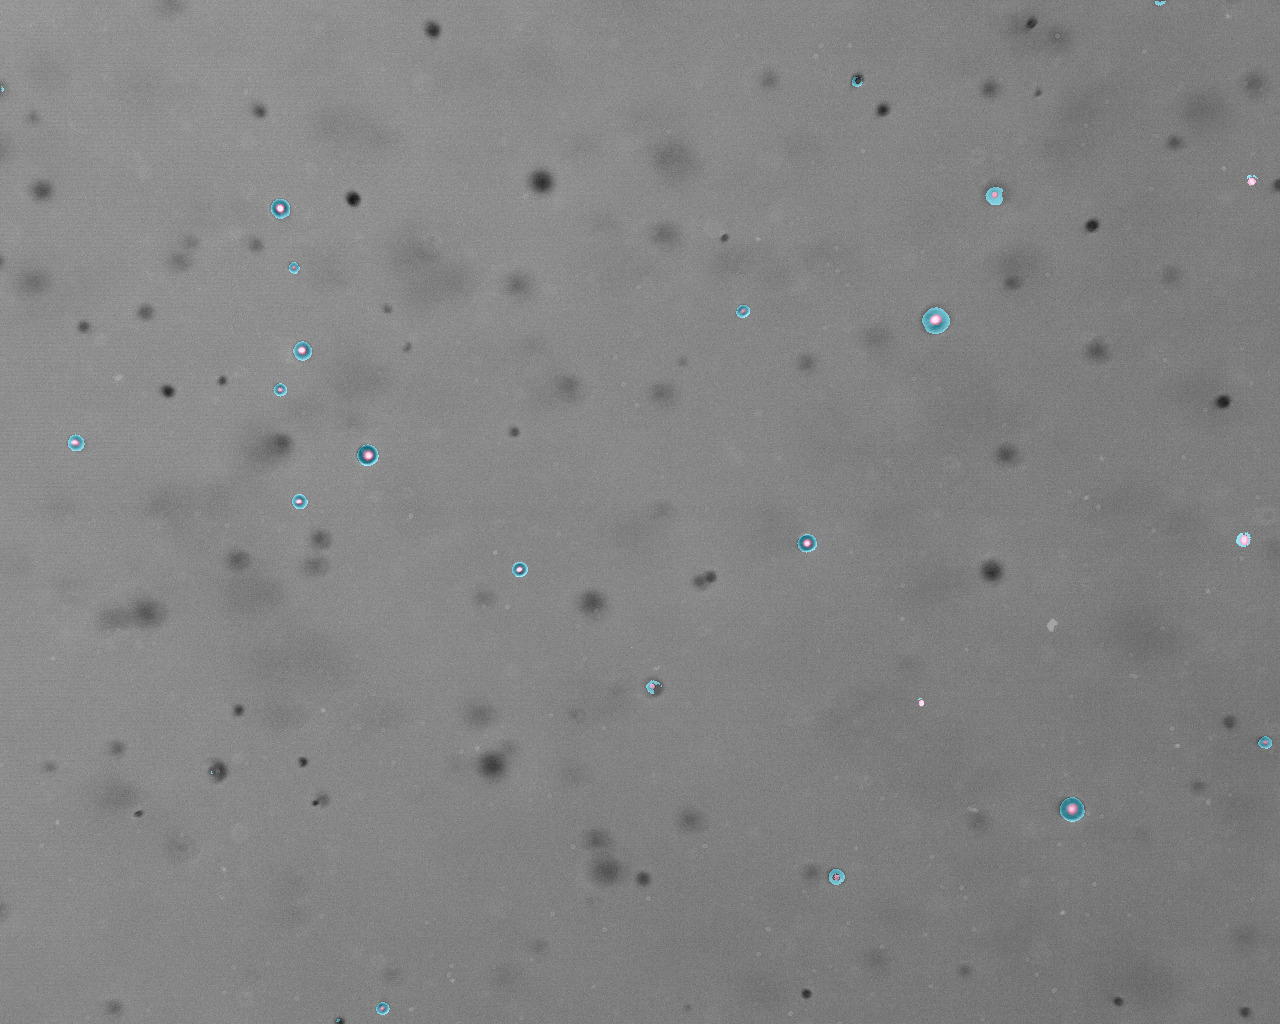
\includegraphics[width=\textwidth]{images/samples/36dbm_C001H001S0001000046_leftImg8bit_overlay.jpeg}
        \caption{Mask overlay for example image 1.}
    \end{subfigure}
\end{figure}
\vfill
~
\vfill
\begin{figure}[htbp]\ContinuedFloat
    \begin{subfigure}{\textwidth}
        \centering
            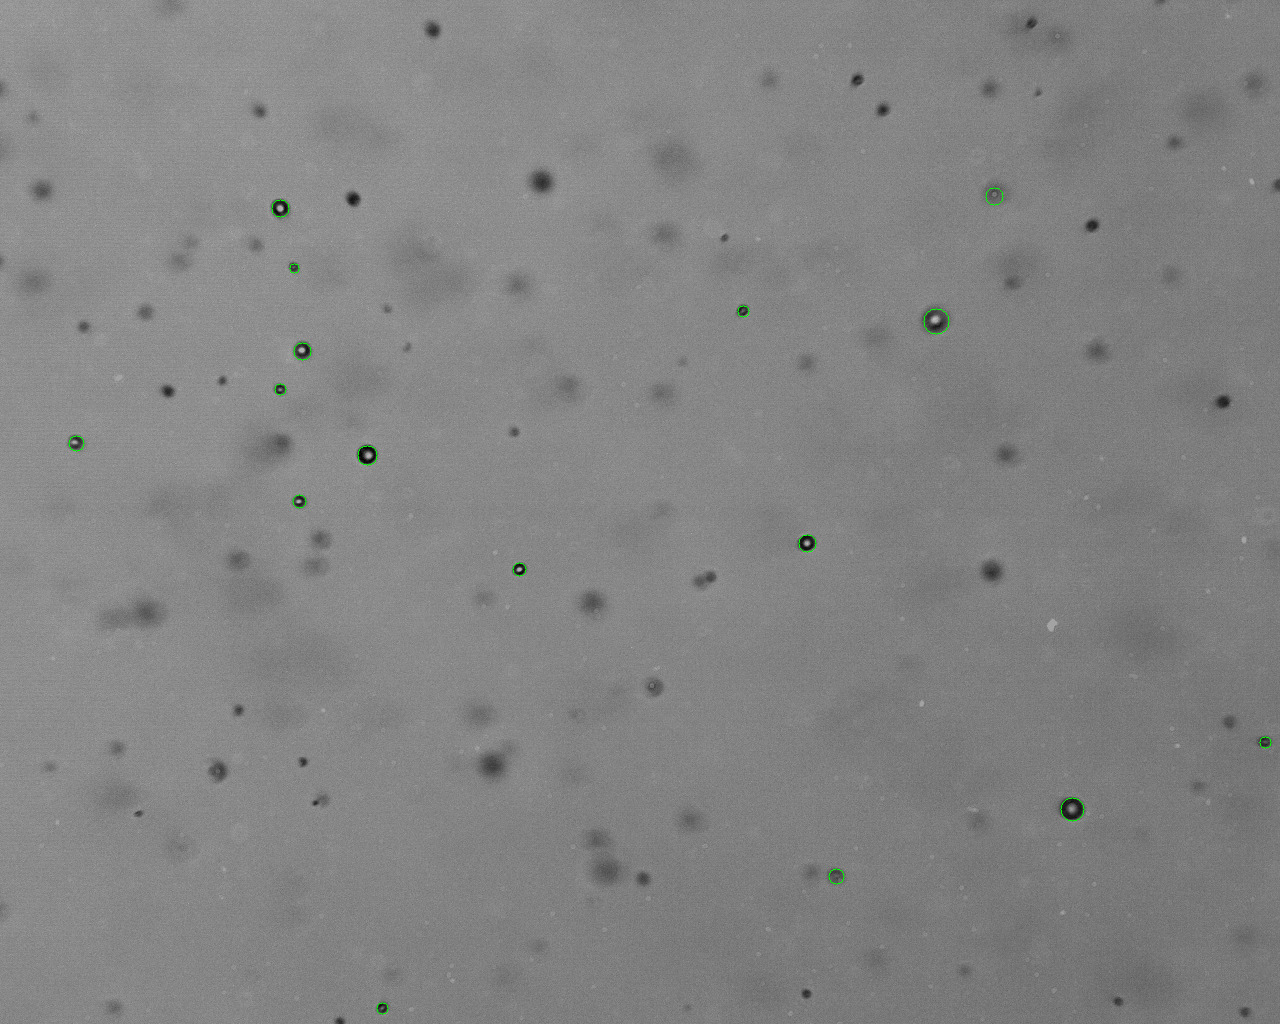
\includegraphics[width=\textwidth]{images/samples/36dbm_C001H001S0001000046_leftImg8bit_detected.jpeg}
        \caption{Detected droplets for example image 1.}
    \end{subfigure}
\end{figure}
~
\vfill
~
\begin{figure}[htbp]\ContinuedFloat
    \centering
    \begin{subfigure}{\textwidth}
        \centering
            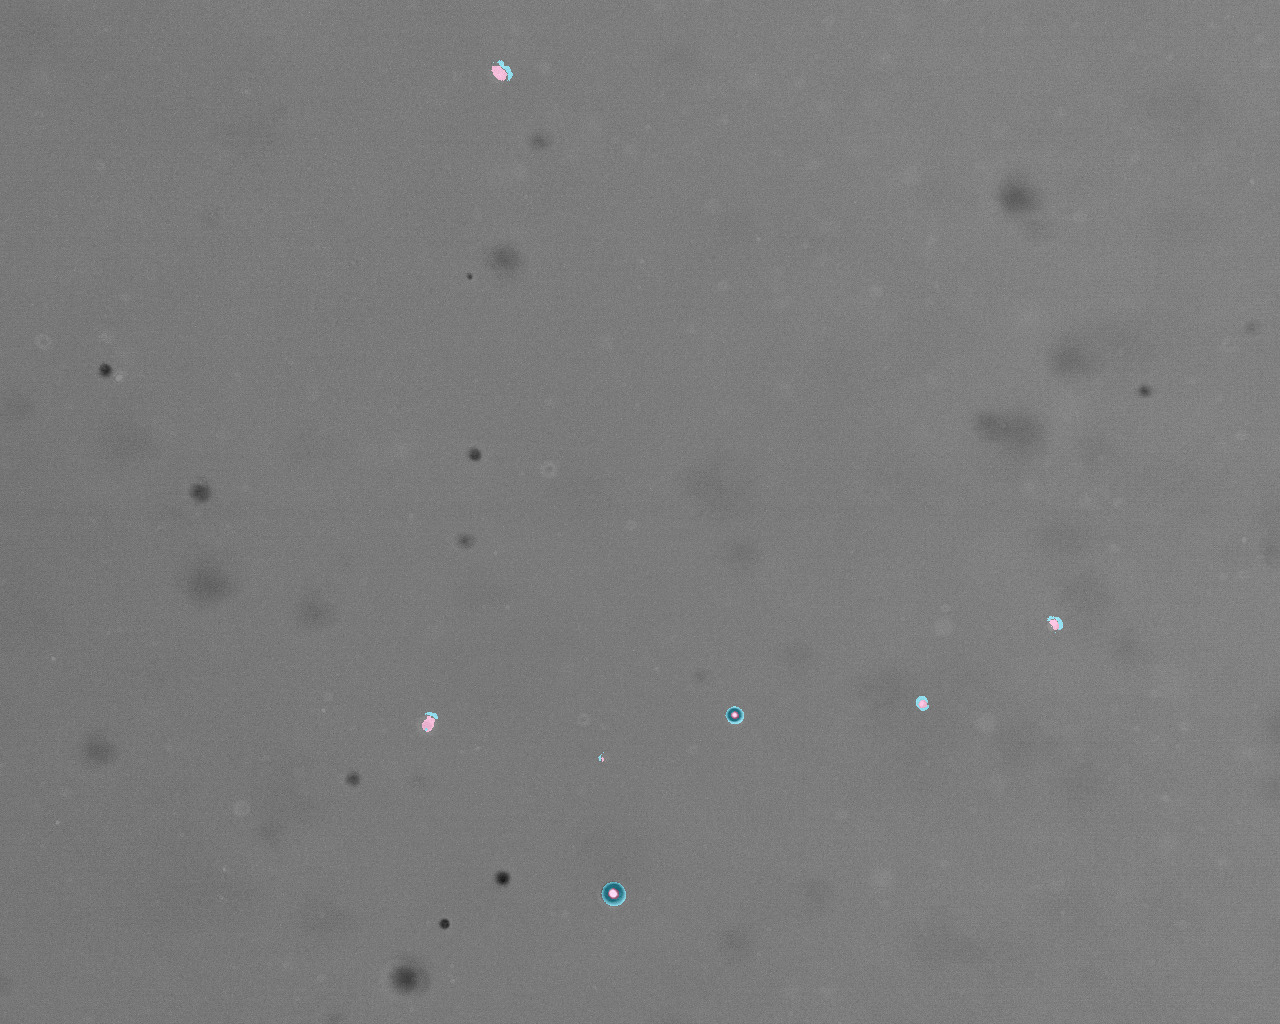
\includegraphics[width=\textwidth]{images/samples/36dbm_C001H001S0001000205_leftImg8bit_overlay.jpeg}
        \caption{Mask overlay for example image 2.}
    \end{subfigure}
\end{figure}
\vfill
~
\vfill
\begin{figure}[htbp]\ContinuedFloat
    \begin{subfigure}{\textwidth}
        \centering
            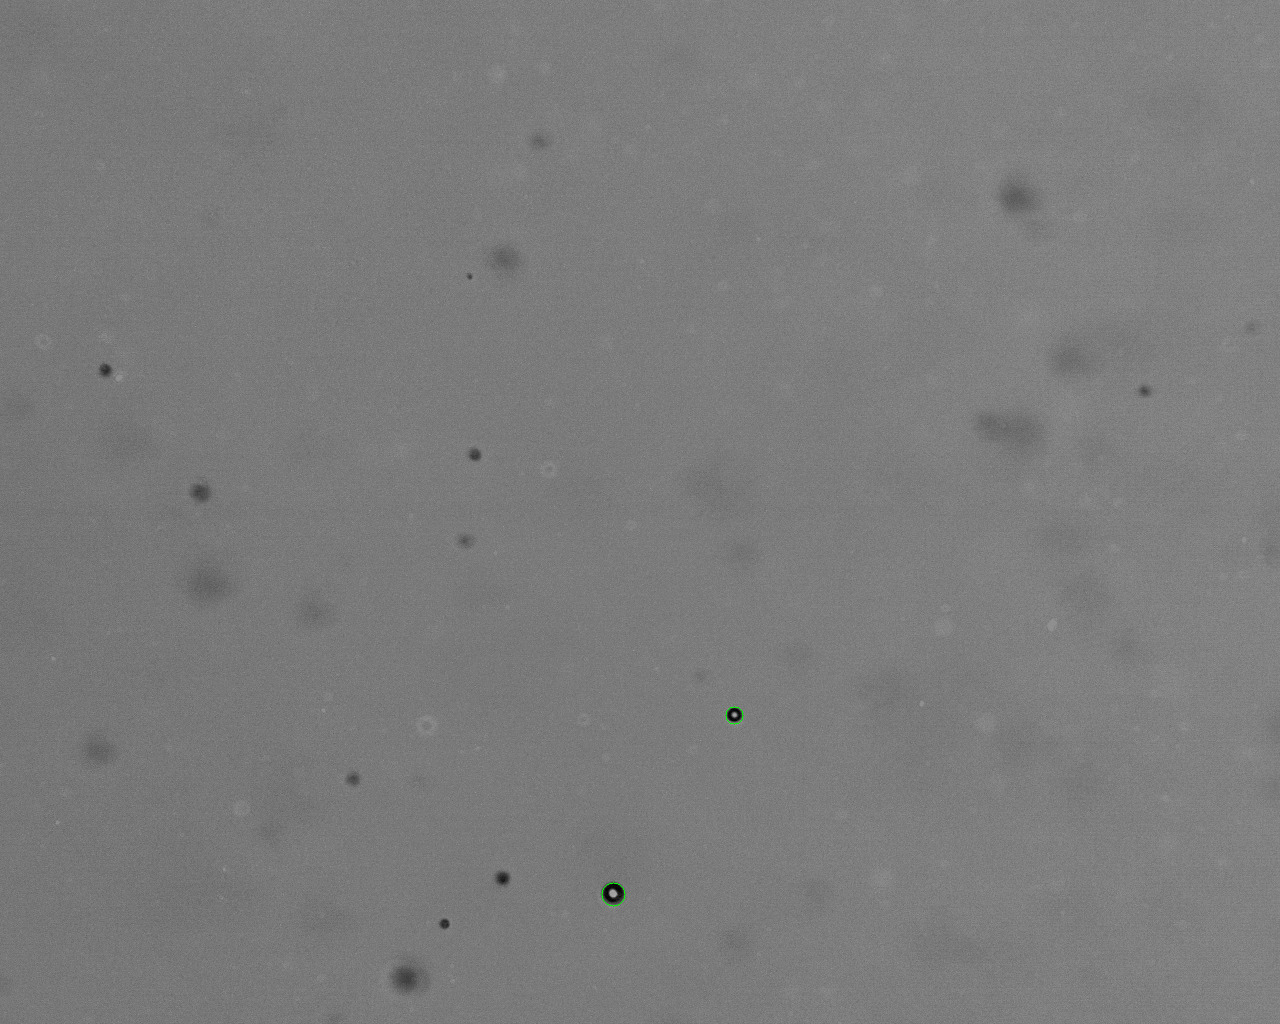
\includegraphics[width=\textwidth]{images/samples/36dbm_C001H001S0001000205_leftImg8bit_detected.jpeg}
        \caption{Detected droplets for example image 2.}
    \end{subfigure}
\end{figure}
~
\vfill
~
\begin{figure}[htbp]\ContinuedFloat
    \centering
    \begin{subfigure}{\textwidth}
        \centering
            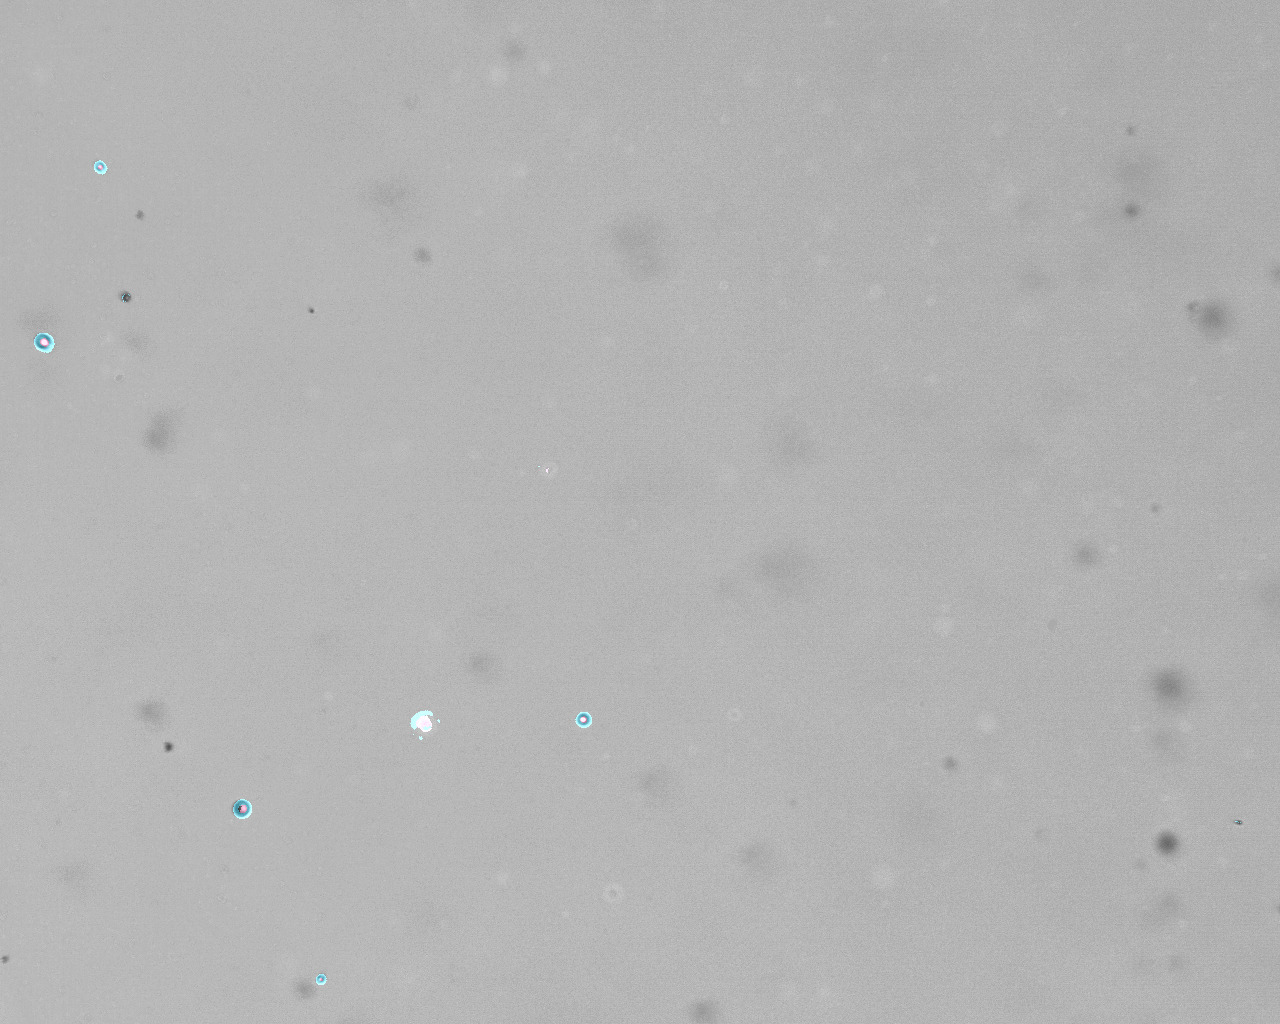
\includegraphics[width=\textwidth]{images/samples/36dbm_C001H001S0001000206_leftImg8bit_overlay.jpeg}
        \caption{Mask overlay for example image 3.}
    \end{subfigure}
\end{figure}
\vfill
~
\vfill
\begin{figure}[htbp]\ContinuedFloat
    \begin{subfigure}{\textwidth}
        \centering
            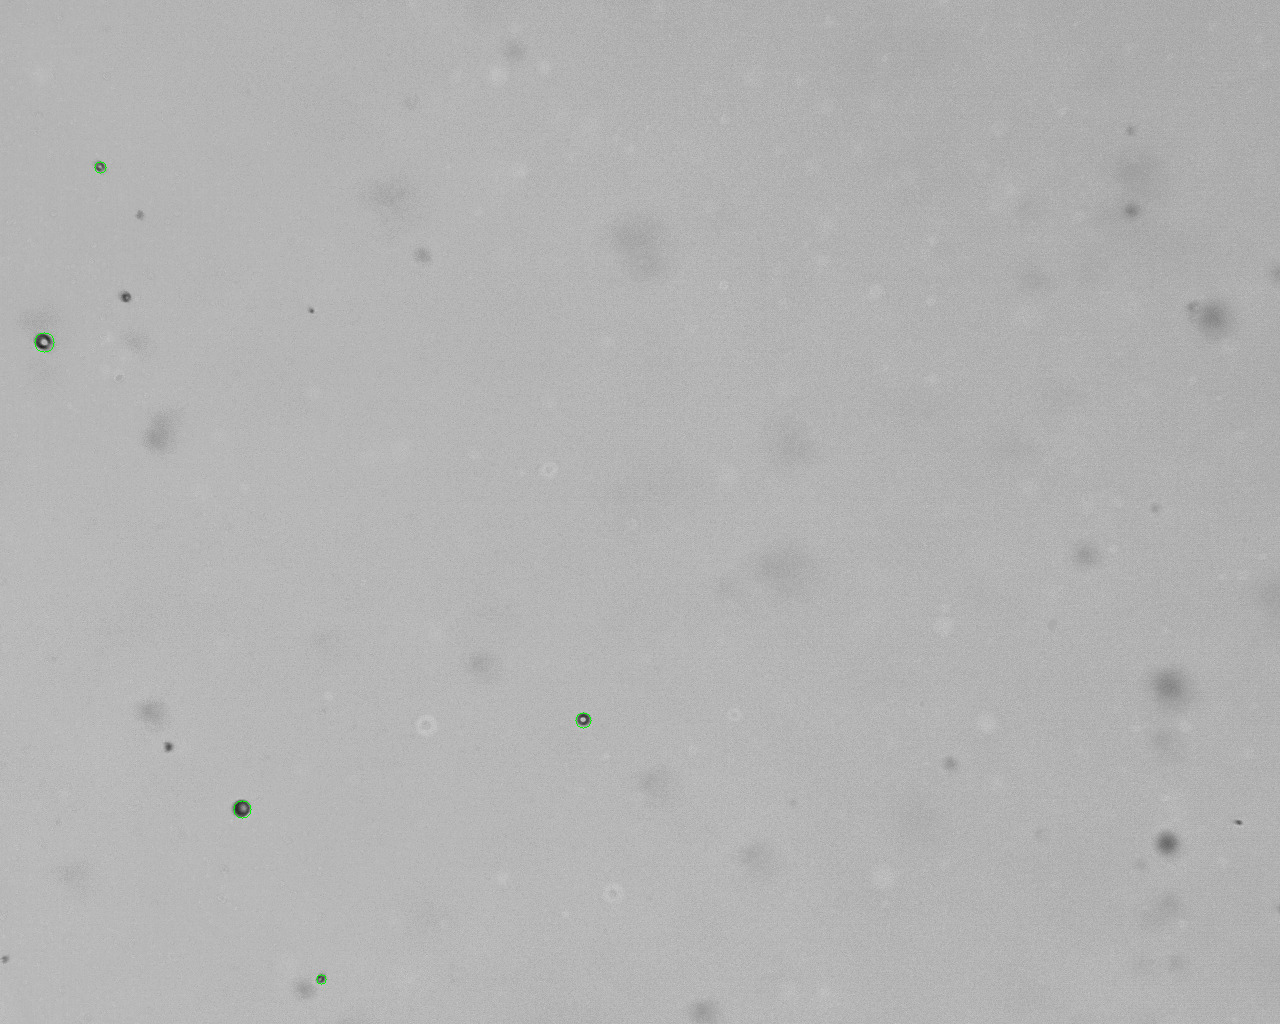
\includegraphics[width=\textwidth]{images/samples/36dbm_C001H001S0001000206_leftImg8bit_detected.jpeg}
        \caption{Detected droplets for example image 3.}
    \end{subfigure}
    \caption{Examples for some of the results from applying the measurement technique developed in the thesis. The images show the overlayed segmentation masks with blue for the droplets border labels and pink for the droplet center labels, as well as the droplets detected after filtering as green circles.}
    \label{fig:example_images}
\end{figure}

    \end{appendices}

\end{document}